\documentclass[8pt]{beamer}
\usetheme{Boadilla}
\usepackage[utf8]{inputenc}
\usepackage{amsmath}
\usepackage{amsfonts}
\usepackage{amssymb}
\usepackage{graphicx}
\usepackage{xcolor}
\author{Adriano Del Vincio}
\usepackage{subfig}
\usepackage[output-decimal-marker={.}]{siunitx}
%\sisetup{detect-all}

\title[Alpha 2]{Toy Model For Hyperfine Measurement}

\setbeamercolor{block title}{fg=white, bg = cyan }
\author[Adriano, Germano, Simone]{Adriano Del Vincio, Germano Bonomi,\\ Simone Stracka}
%\setbeamercovered{transparent} 
%\setbeamertemplate{navigation symbols}{} 
\logo{
\includegraphics[width = 0.125\textwidth]{../../../logo/ALPHA_Logo.jpg}}
\newcommand{\nologo}{\setbeamertemplate{logo}{}}
\institute[]{University of Brescia, INFN Pisa} 
\titlegraphic{
\begin{figure}
\hspace{1.cm}

\includegraphics[width = 0.12\textwidth ]{../../../logo/logounibs.png}
%\hspace{1cm}

\includegraphics[width = 0.25\textwidth ]{../../../logo/1_Pisa_LOGO_SIGLA.pdf}
\end{figure}
} 
\beamertemplatenavigationsymbolsempty
\begin{document}

\begin{frame}
\titlepage
\end{frame}

%\begin{frame}
%\tableofcontents
%\end{frame}

\begin{frame}{Scheme of the Simulation}
Scheme of the Monte Carlo Toy for generating the events

\begin{figure}
\centering
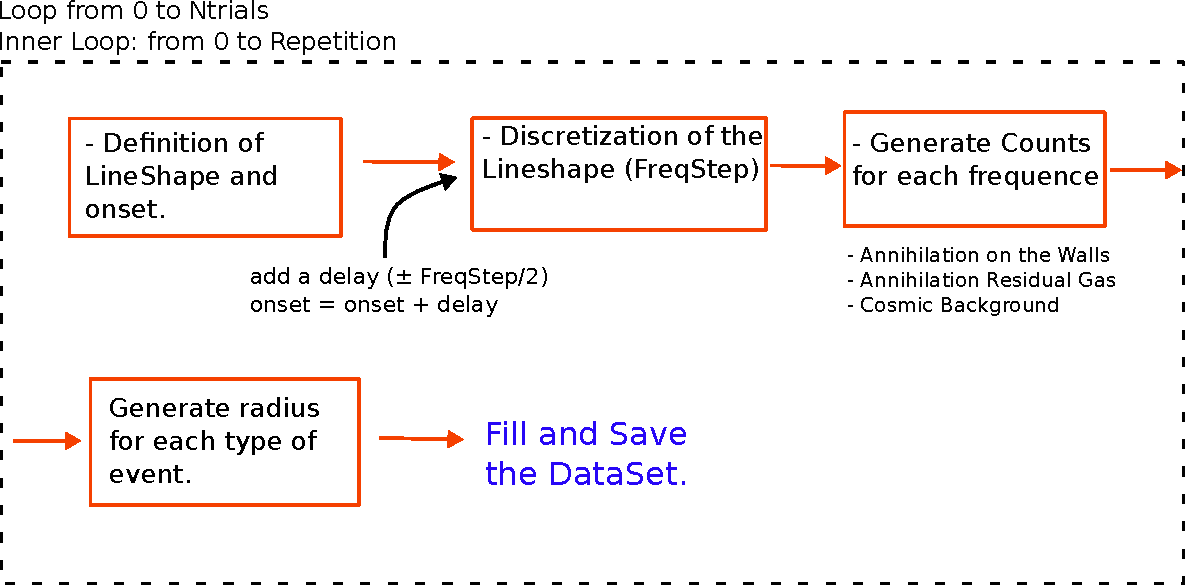
\includegraphics[width = 0.95\textwidth]{SimulationScheme.pdf}
\end{figure}

\begin{center}
In this simulation, the data are created and analyzed using\newline \textit{RDataFrame} framework.
\end{center}

\end{frame}

\begin{frame}{A brief introduction about the Monte Carlo}

We have developed a Monte Carlo Toy that produces two \texttt{.root} dataset files. The variables are columns of values that are shown in the figure below:
\begin{figure}[hbtp]
 \centering
 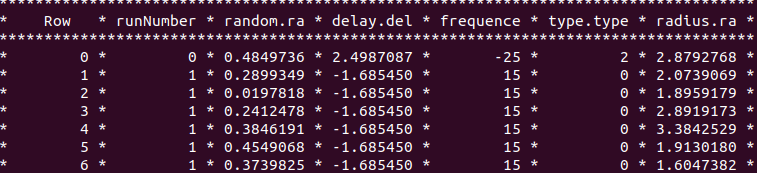
\includegraphics[width = 0.75\textwidth]{DatasetContent.png}
 \caption{ Structure of the dataset.}
 \end{figure}

\begin{itemize}
\item \textit{runNumber}: identifies which run the event belong to (from $0$ to $Repetition -1$) 
\item \textit{random}: values uniform distributed from $0$ to $1$, can be used to randomize the selection or for sub-sampling in the data
\item \textit{shift}: store the onset shift
\item \textit{frequence}: the frequency of the event
\item \textit{type}: type of the event: 0 annihilation on the walls, 1 residual gas annihilation, 2 cosmic event
\item \textit{radius}: radius of the annihilation vertex.
\end{itemize}

\end{frame}

\begin{frame}{A brief introduction about the Monte Carlo}

The Annihilation on the walls are generated as function of the frequency, using the two line-shapes of the transitions (c $\rightarrow$ b) and (d $\rightarrow$ a). The Annihilation on the residual gas and the cosmic background are generated uniformly on the frequency spectrum. All the parameters of the simulation are loaded from the \texttt{ToyConfiguration.txt} file. The parameters are chosen to reproduce the runs 4b.

\begin{figure}[hbtp]
\centering
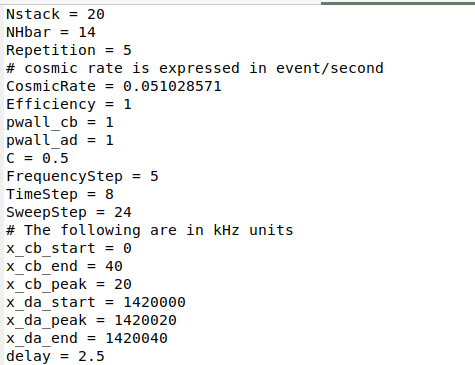
\includegraphics[width = 0.5\textwidth]{MontecarloParams.png}
\caption{ Parameters of the Toy.}
\end{figure}
\end{frame}

\begin{frame}{Triangular Line-shape Pdfs}

For this first use of the toy, we have chosen simple line-shapes, triangular with a symmetric rise and fall.

\begin{figure}
\centering
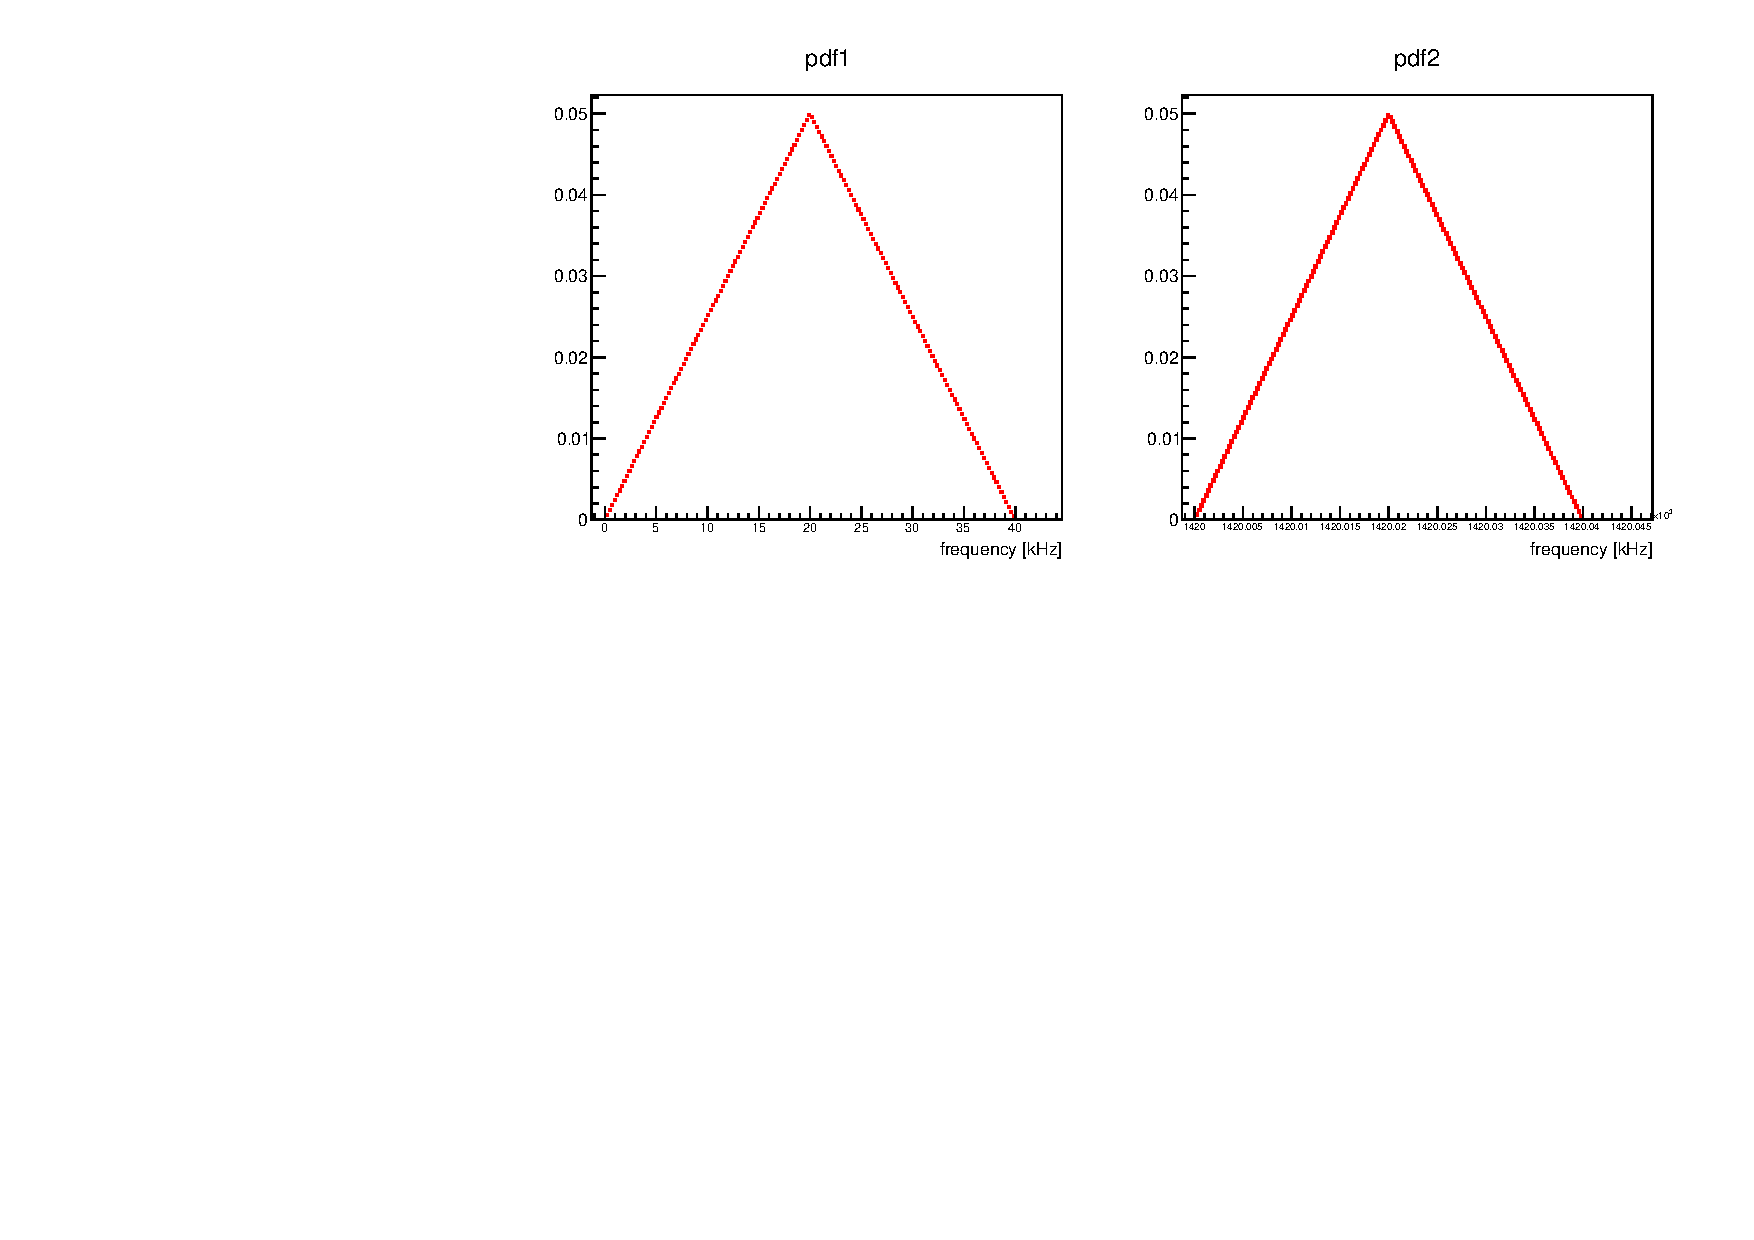
\includegraphics[width = \textwidth]{../Plot/Pdf1Pdf2.pdf}
\end{figure}

\end{frame}

\begin{frame}{Triangular Line-shapes Simulation}

We sample at the given frequency step of $\SI{5}{ \kilo \hertz}$ the Pdfs, to simulate the experimental line-shapes. We applied the onset finding algorithm to this distribution.
 
\begin{figure}
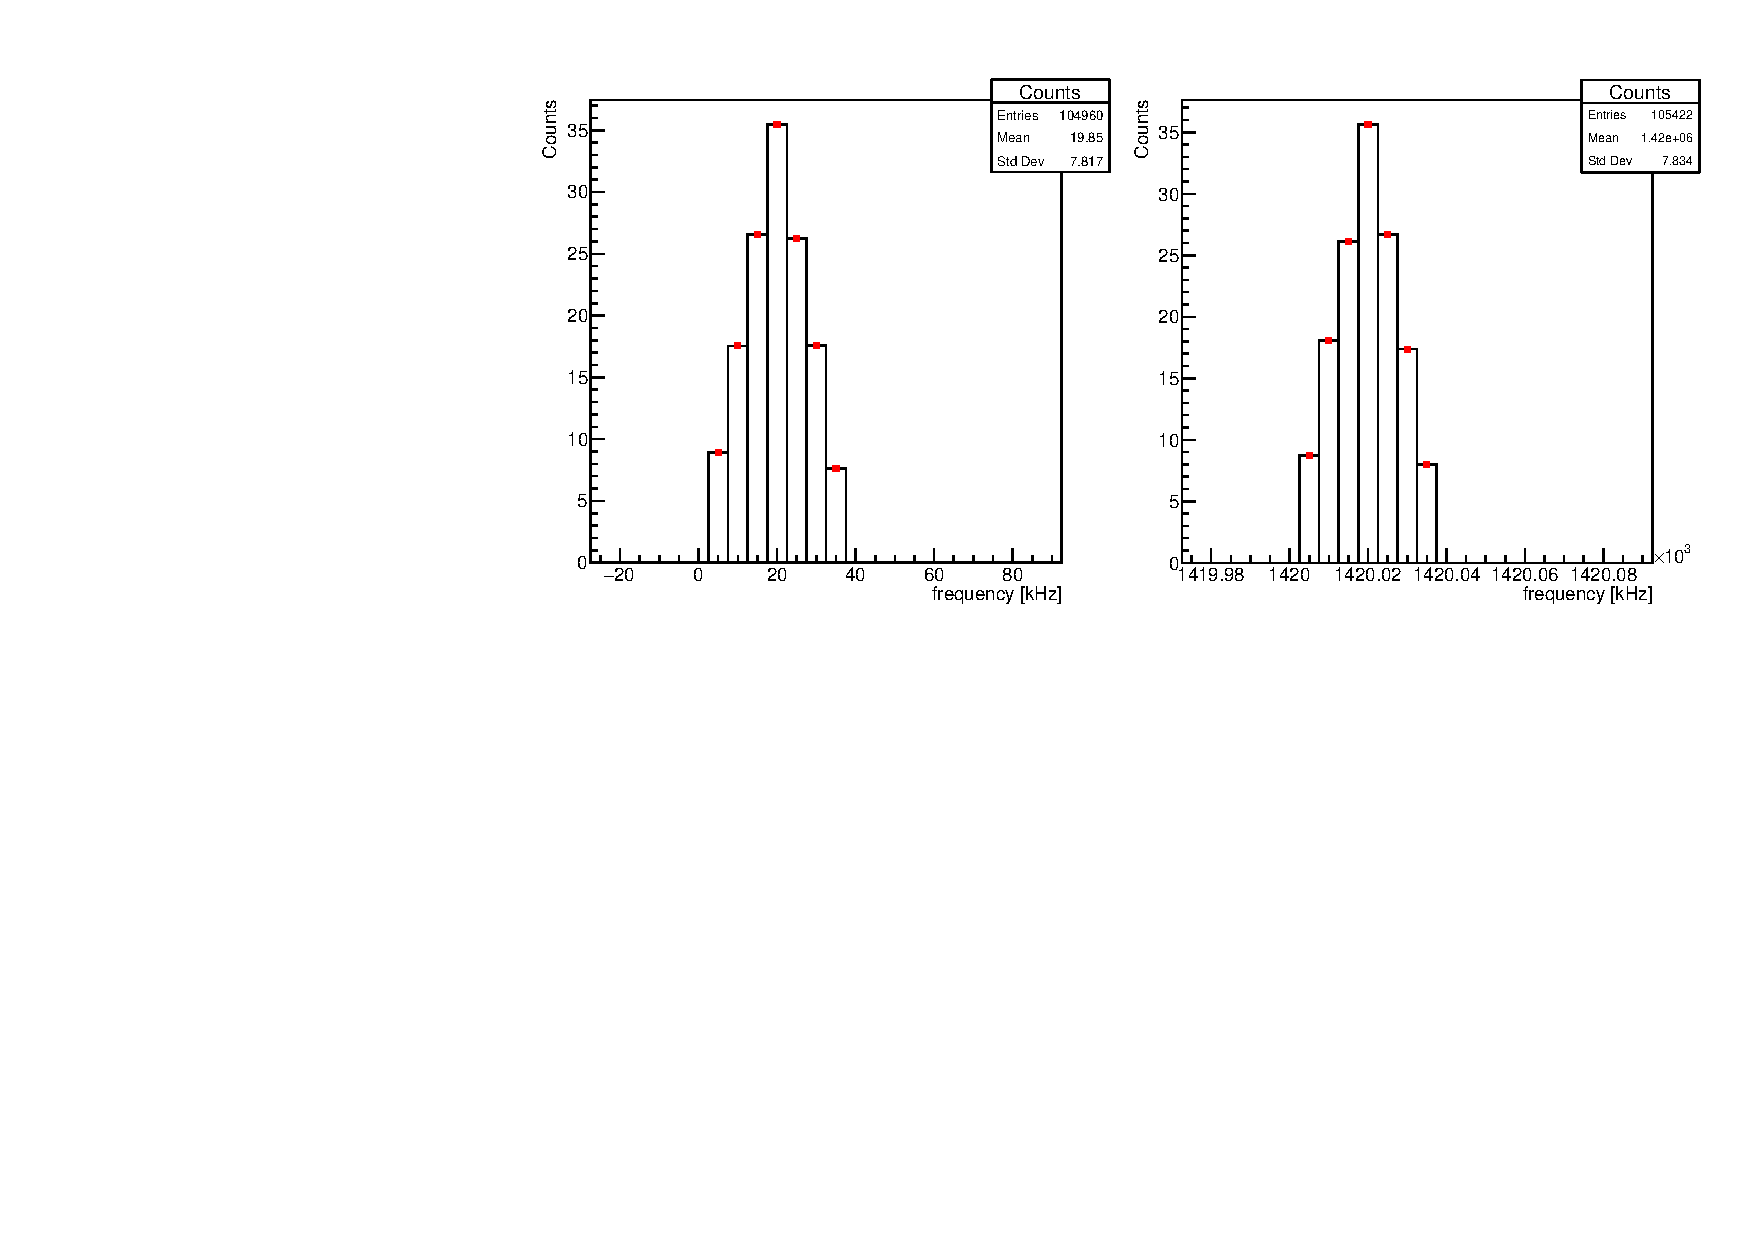
\includegraphics[width = \textwidth]{TriangleLineShape.pdf}
\end{figure}

The onset is fixed ad $f = \SI{0}{\kilo \hertz}$. In this sample the cosmic background is\newline set to zero.

\end{frame}

\begin{frame}{A simple Onset finding Algorithm}

The first algorithm that is tested is quite simple: {\color{red}{ \textbf{the onset is identified by the first bin with a content over a given threshold}} ($> N\mu_{cosmic}$)} \footnote{Where the $\mu_{cosmic}$ is computed from the Poisson distribution of the cosmic counts expected per bin.}

Before showing the plot with the simulated data, it is useful to remind how this algorithm deals with the frequency step:

\begin{figure}
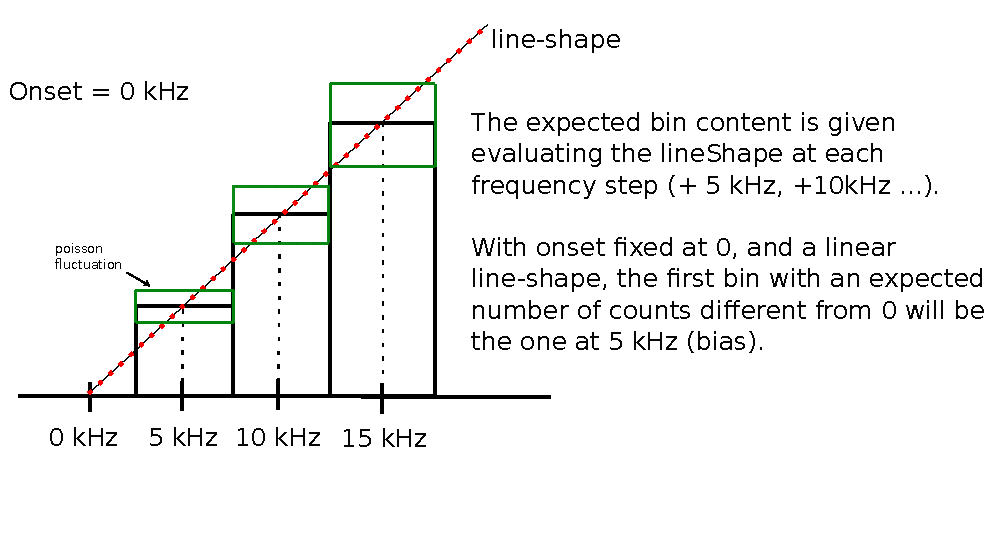
\includegraphics[width = 0.9\textwidth]{ExplainingAlgorithm1.pdf}
\end{figure}
\end{frame}

\begin{frame}{Consistency Check 1}

We have tested the algorithm with a dataset without cosmic background and shift fixed to zero. The algorithm identifies the onset at frequency $\SI{5}{\kilo \hertz}$.

\begin{figure}
\includegraphics[width = 0.9\textwidth]{../Plot/OnsetResult.pdf}
\end{figure} 
\end{frame}

\begin{frame}{Consistency Check 2}

We have tested the algorithm with a dataset without cosmic background. The shift is uniform distributed in $\SI{-2.5}{\kilo \hertz}$ and $\SI{+2.5}{\kilo \hertz}$.

\begin{figure}
\includegraphics[width = 0.9\textwidth]{../Plot/OnsetResult7.pdf}
\end{figure} 

With the shift, two bins ( $frequency = \SI{0}{\kilo \hertz}$ and $frequency = \SI{5}{\kilo \hertz}$) are populated.
\end{frame}

\begin{frame}{Consistency Check 2}


\begin{figure}
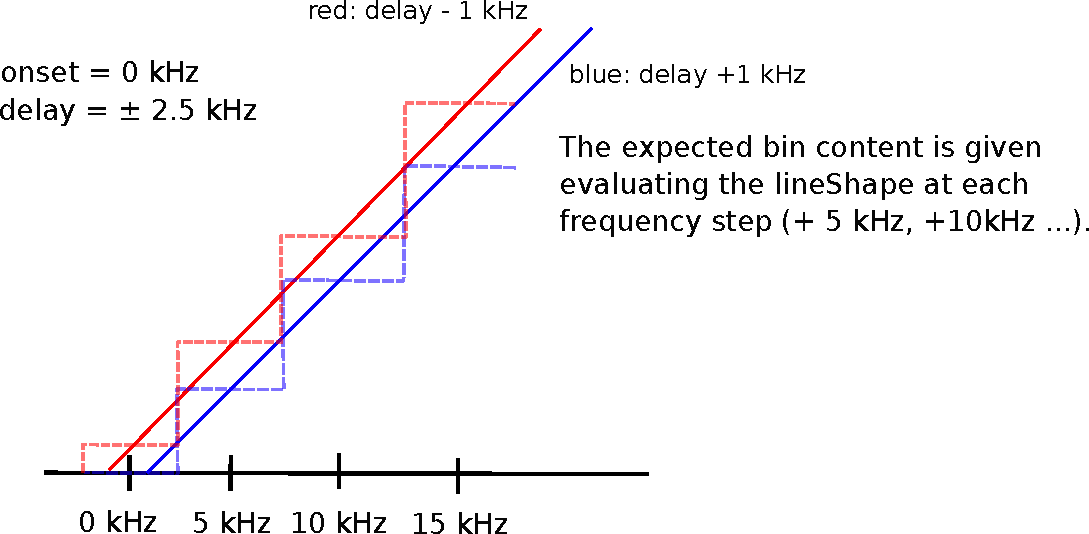
\includegraphics[width = 0.8\textwidth]{ExplainingAlgorithm2.pdf}
\end{figure}

The frequency step are fixed, and the lineshape is shifted accordingly to the extracted value of the shift. In few words:
\begin{itemize}
\item step 1): fix the frequency steps (the frequency effectively used in the experiment)
\item step 2): define the new value of the onset adding a uniform distributed shift  
\item step 3): shift the lineshape accordingly to the new value of the onset,\newline discretize the lineshape and proceed with the generation of the data.
\end{itemize}
\end{frame}

\begin{frame}{algorithm test: threshold $ > 3 \mu_{cosmic}$}

In this case, we have applied the algorithm to simulated data with cosmic background (using a rate of $0.051 \frac{event}{s}$, from passcut1). Each bin has an expected cosmic background of $dwelltime \cdot rate = 0.408$.
The shift is uniform distributed in $\SI{-2.5}{\kilo \hertz}$ and $\SI{+2.5}{\kilo \hertz}$. 
\begin{figure}
\includegraphics[width = 0.9\textwidth]{../Plot/OnsetResult11.pdf}
\end{figure}
\end{frame}

\begin{frame}{algorithm test: threshold $ > 5 \mu_{cosmic}$}

In this case, we have applied the algorithm to simulated data with cosmic background (using a rate of $0.051 \frac{event}{s}$, from passcut1). Each bin has an expected cosmic content of $dwelltime \cdot rate = 0.408$.
The shift is uniform distributed in $\SI{-2.5}{\kilo \hertz}$ and $\SI{+2.5}{\kilo \hertz}$. 
\begin{figure}
\includegraphics[width = 0.9\textwidth]{../Plot/OnsetResult12.pdf}
\end{figure}

\end{frame}


\begin{frame}{algorithm test: threshold $ > 8 \mu_{cosmic}$}

In this case, we have applied the algorithm to simulated data with cosmic background (using a rate of $0.051 \frac{event}{s}$, from passcut1). Each bin has an expected cosmic content of $dwelltime \cdot rate = 0.408$.
The shift is uniform distributed in $\SI{-2.5}{\kilo \hertz}$ and $\SI{+2.5}{\kilo \hertz}$. 
\begin{figure}
\includegraphics[width = 0.9\textwidth]{../Plot/OnsetResult15.pdf}
\end{figure}

\end{frame}

\begin{frame}{ Improvements of the week (30/11 - 07/12)}
\begin{itemize}
\item Implemented the onset-finding algorithm of 2017 ($first > 0 , second > 1$)
\item Simulation with a lineShape following the \texttt{ run 69373 } (lineShape with high statistics).
\item Implementation and test of different onset finding algorithms.
\end{itemize}
\end{frame}

\begin{frame}{Fit to the data of run 69373}

The lineShape is fitted using a Cruijff function, which takes into account the asymmetry of the left-right tails, ($model = N \cdot exp(  \frac{-(x - x_{0})^2}{2\sigma_{0,1} + k_{0,1}(x - x_{0})^{2}})$) 

\begin{figure}[hbtp]
\centering
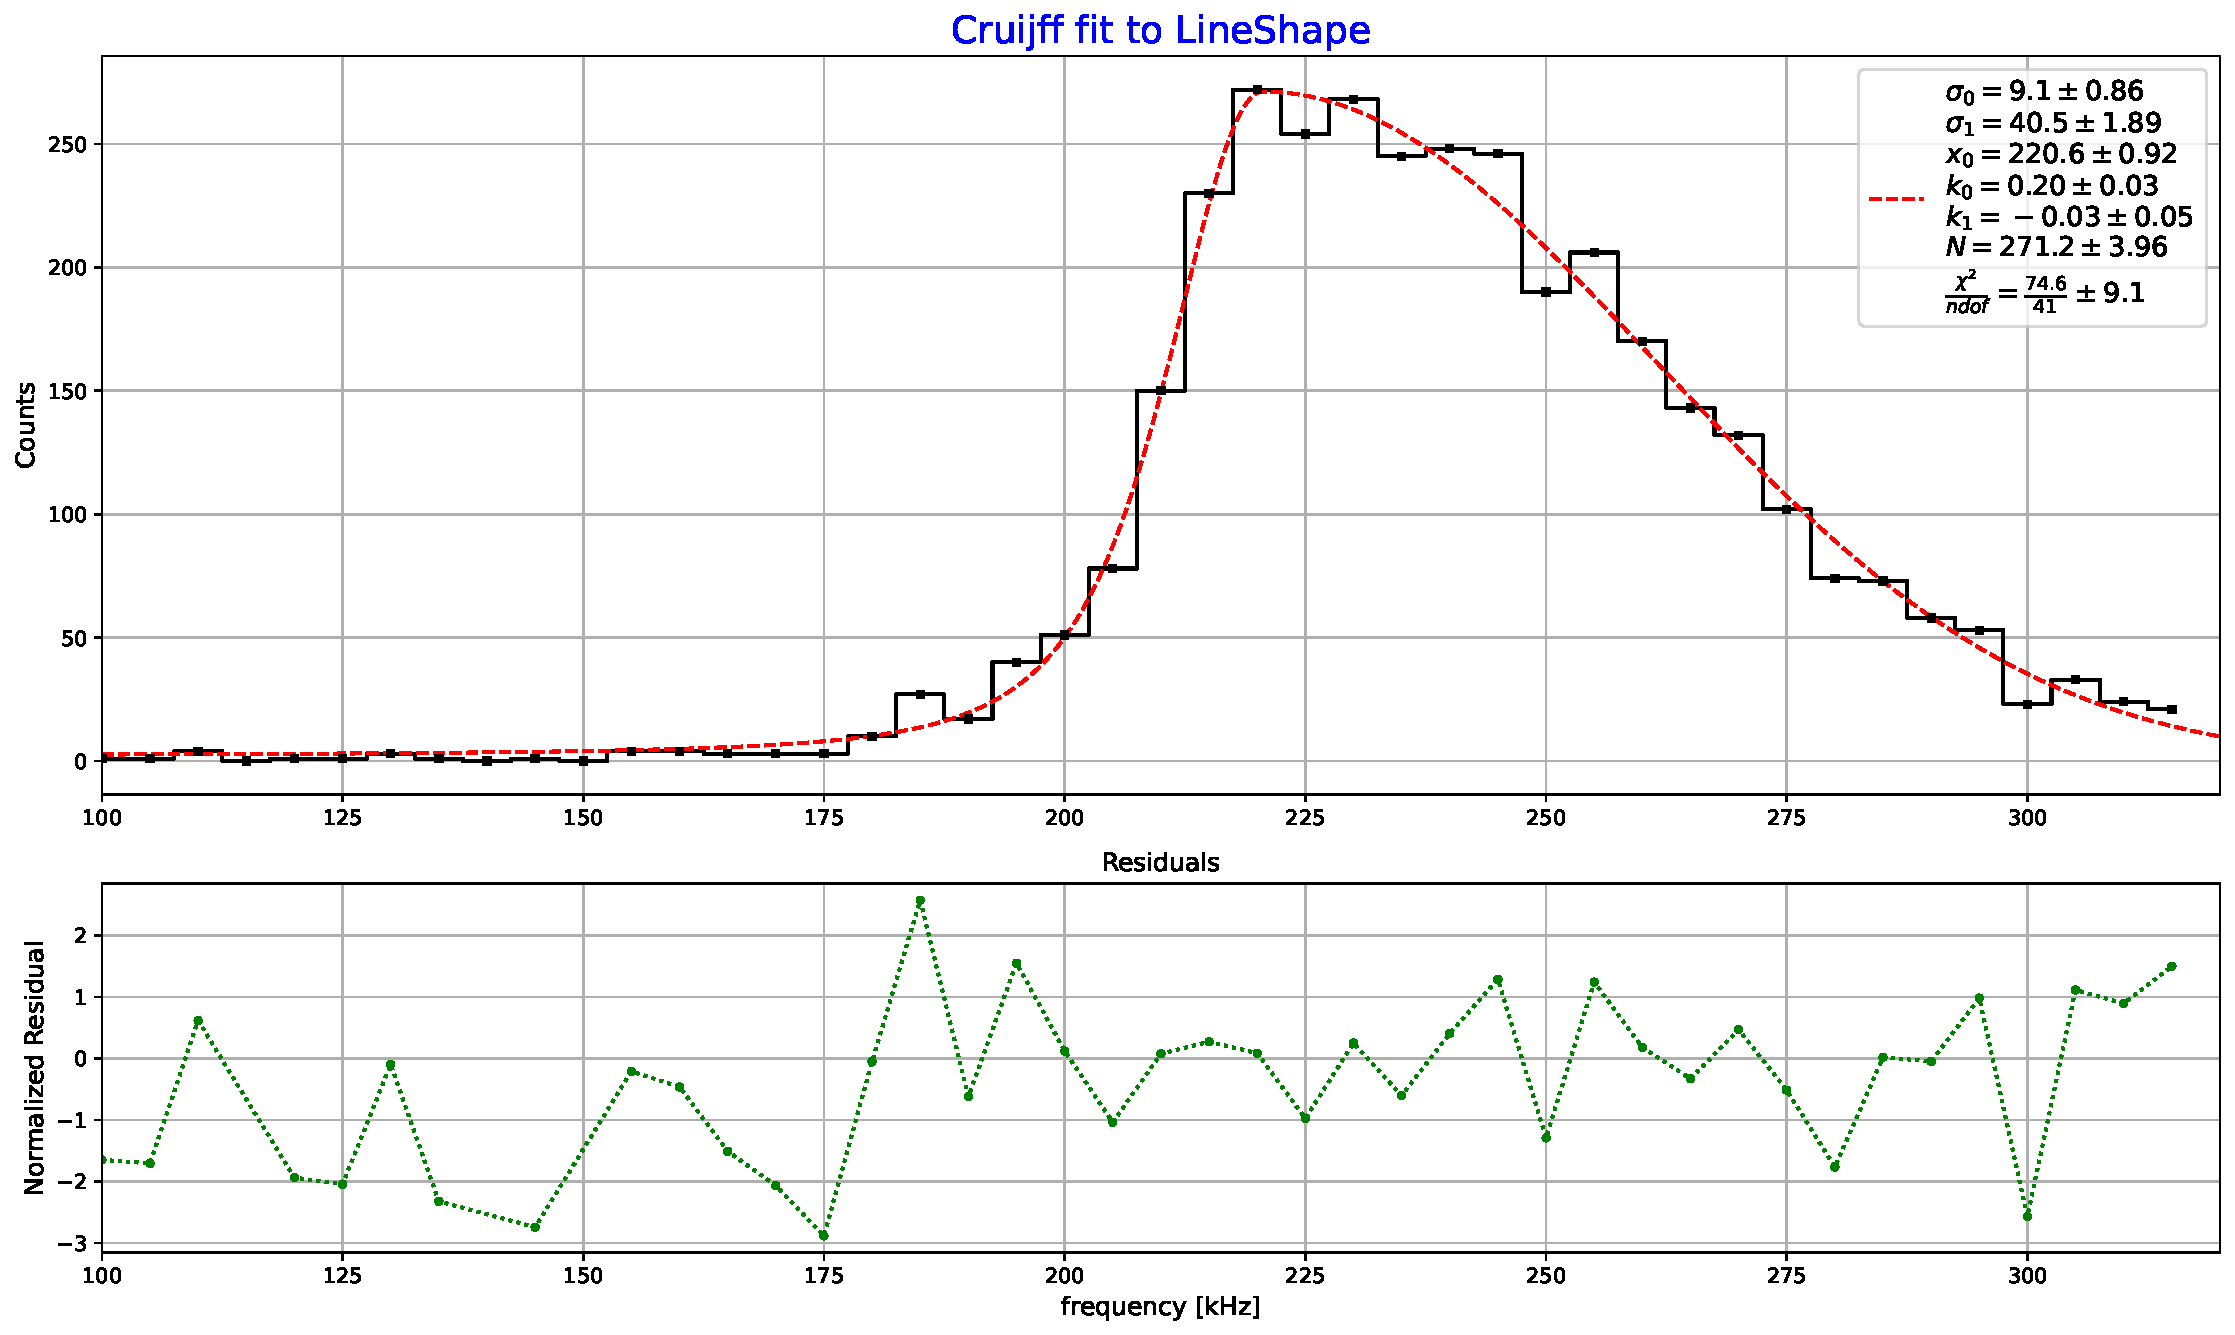
\includegraphics[width = 0.8\textwidth ]{../Plot/FitToLineShape.pdf}
\caption{On top plot, the black line represents data and the red line the fit with the\newline Cruijff function.}
\end{figure}
\end{frame}

\begin{frame}

The Cruijff function is used in the simulation to generate the data. \textbf{The Cruijff is truncated at $f_{0} = \SI{175}{\kilo \hertz}$}. In this way the onset of the lineshape is unambiguously determined. The new model is:

\begin{equation}
model =
\begin{cases}
baseline 	& f \leqslant \SI{175}{\kilo \hertz} \\
N \cdot exp(  \frac{-(x - x_{0})^2}{2\sigma_{0} + k_{0}(x - x_{0})^{2}}) & \SI{175}{\kilo \hertz} < f \leqslant x_{0} \\
N \cdot exp(  \frac{-(x - x_{0})^2}{2\sigma_{1} + k_{1}(x - x_{0})^{2}}) &  f >  x_{0}
\end{cases}
\end{equation}

\begin{figure}[hbtp]
\centering
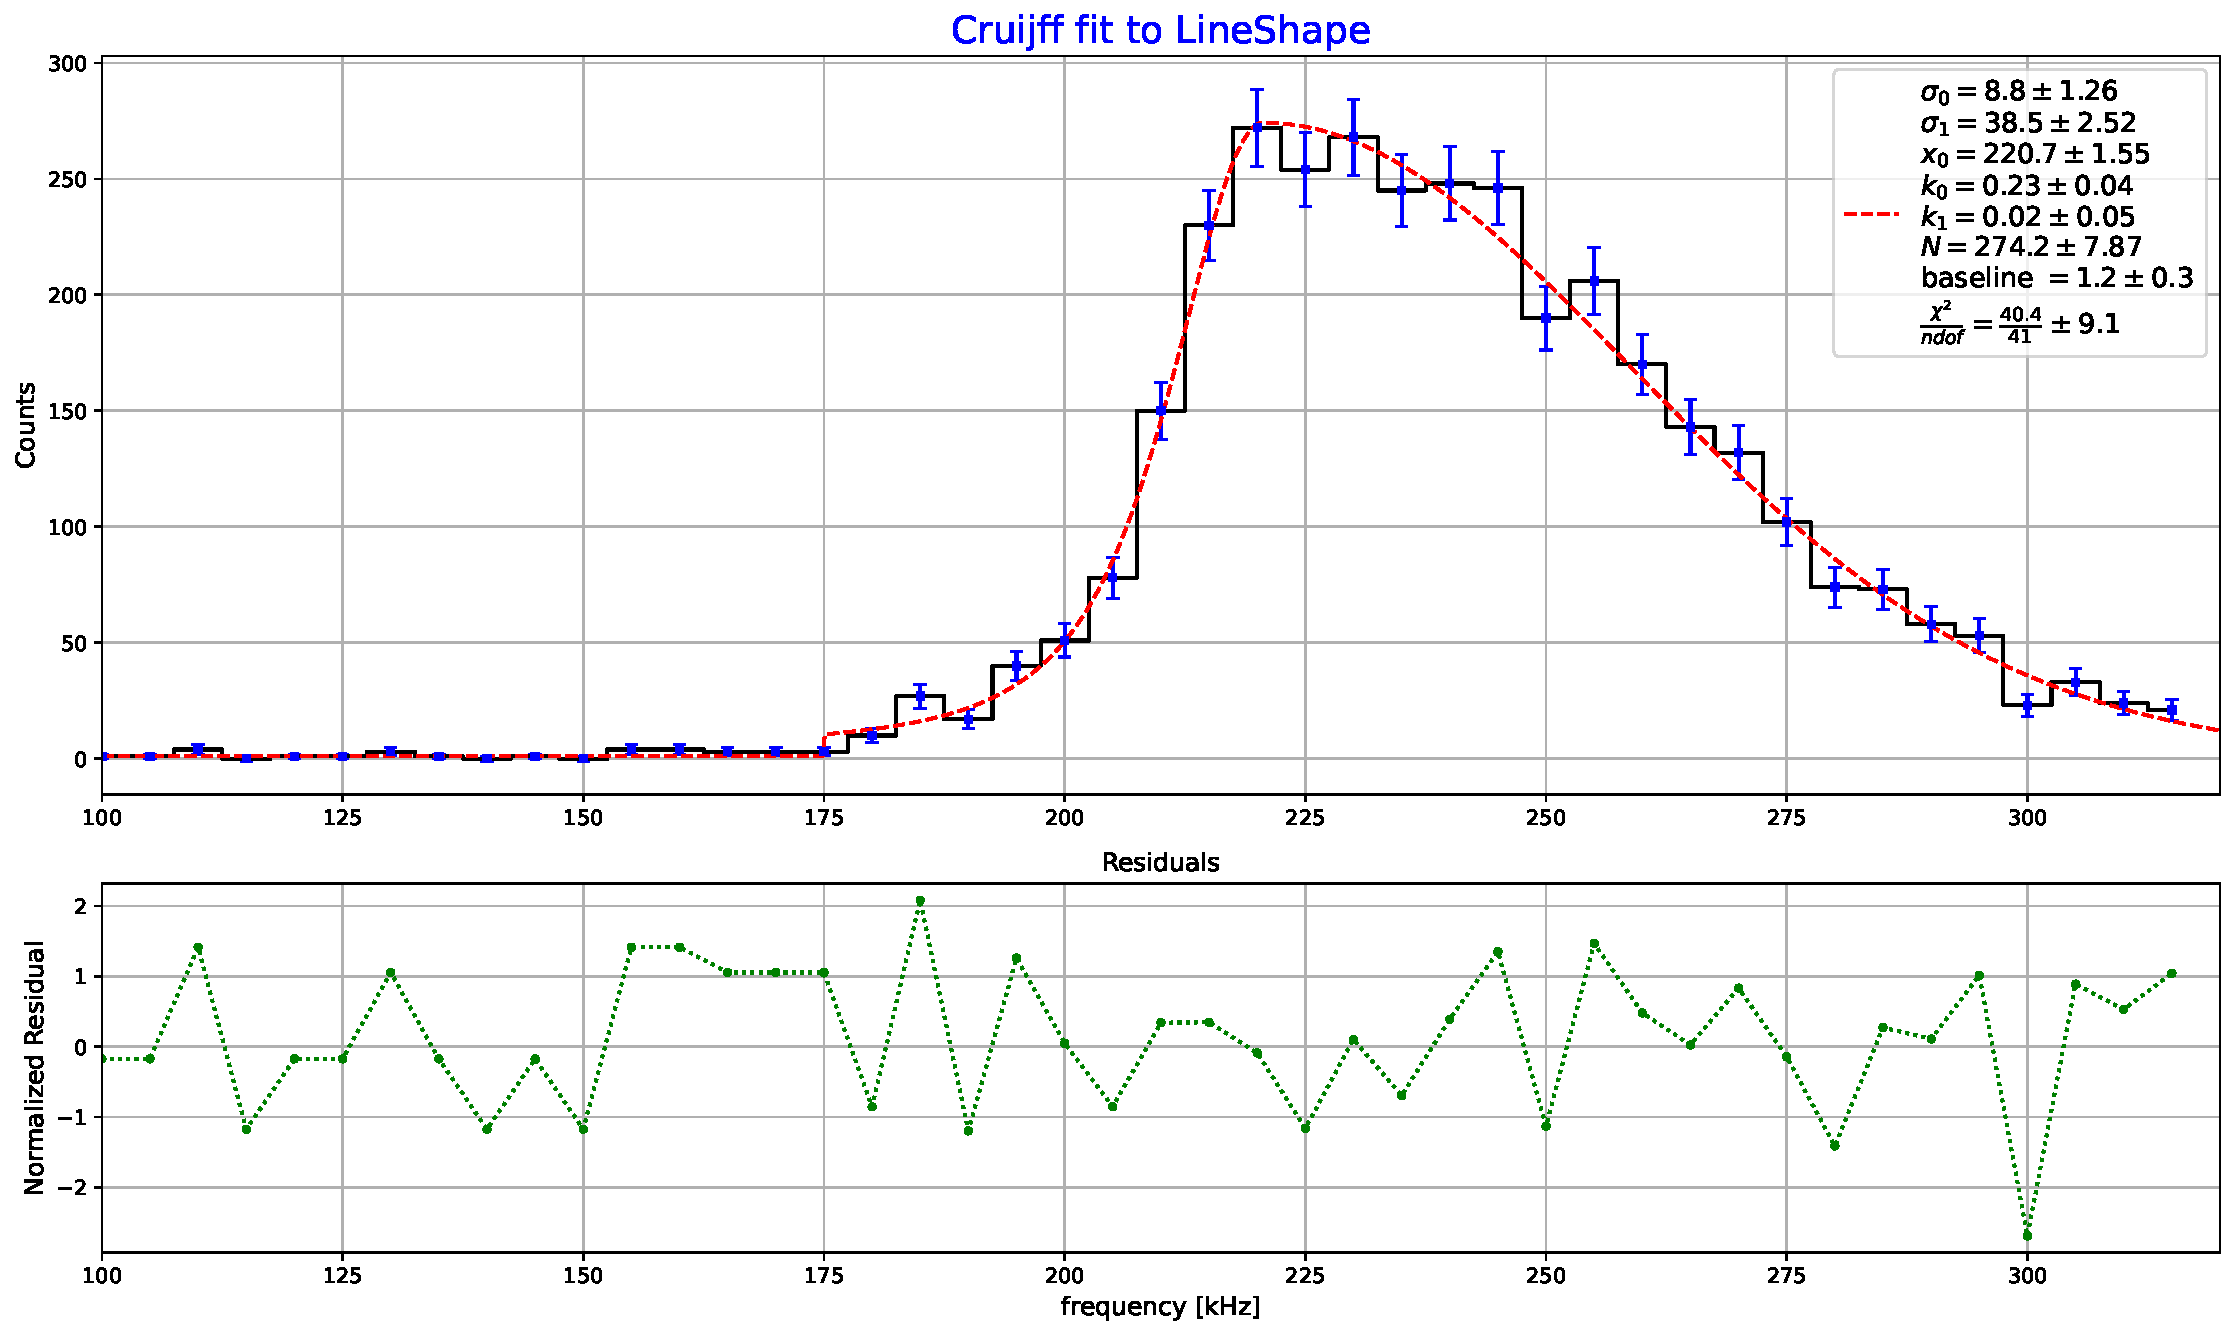
\includegraphics[width = 0.75\textwidth]{../Plot/TruncatedLineShape.pdf}
%\caption{ Fit with a truncated Cruijff function at $ f = \SI{175}{\kilo \hertz}$}
\end{figure}

\textit{Is the baseline compatible with the Cosmic Background?}
\end{frame}

{\nologo
\begin{frame}{Discretization of the lineshape}

Here we plot the discretized lineshape, obtained sampling the Cruijff function with the optimal parameters by the fit of the previous slide. The lineshape is discretized into a series of 50 points, with a increment step of $\SI{5}{\kilo \hertz}$. The starting frequence is $f = \SI{160}{\kilo \hertz}$ 

\begin{figure}[hbtp]
\centering
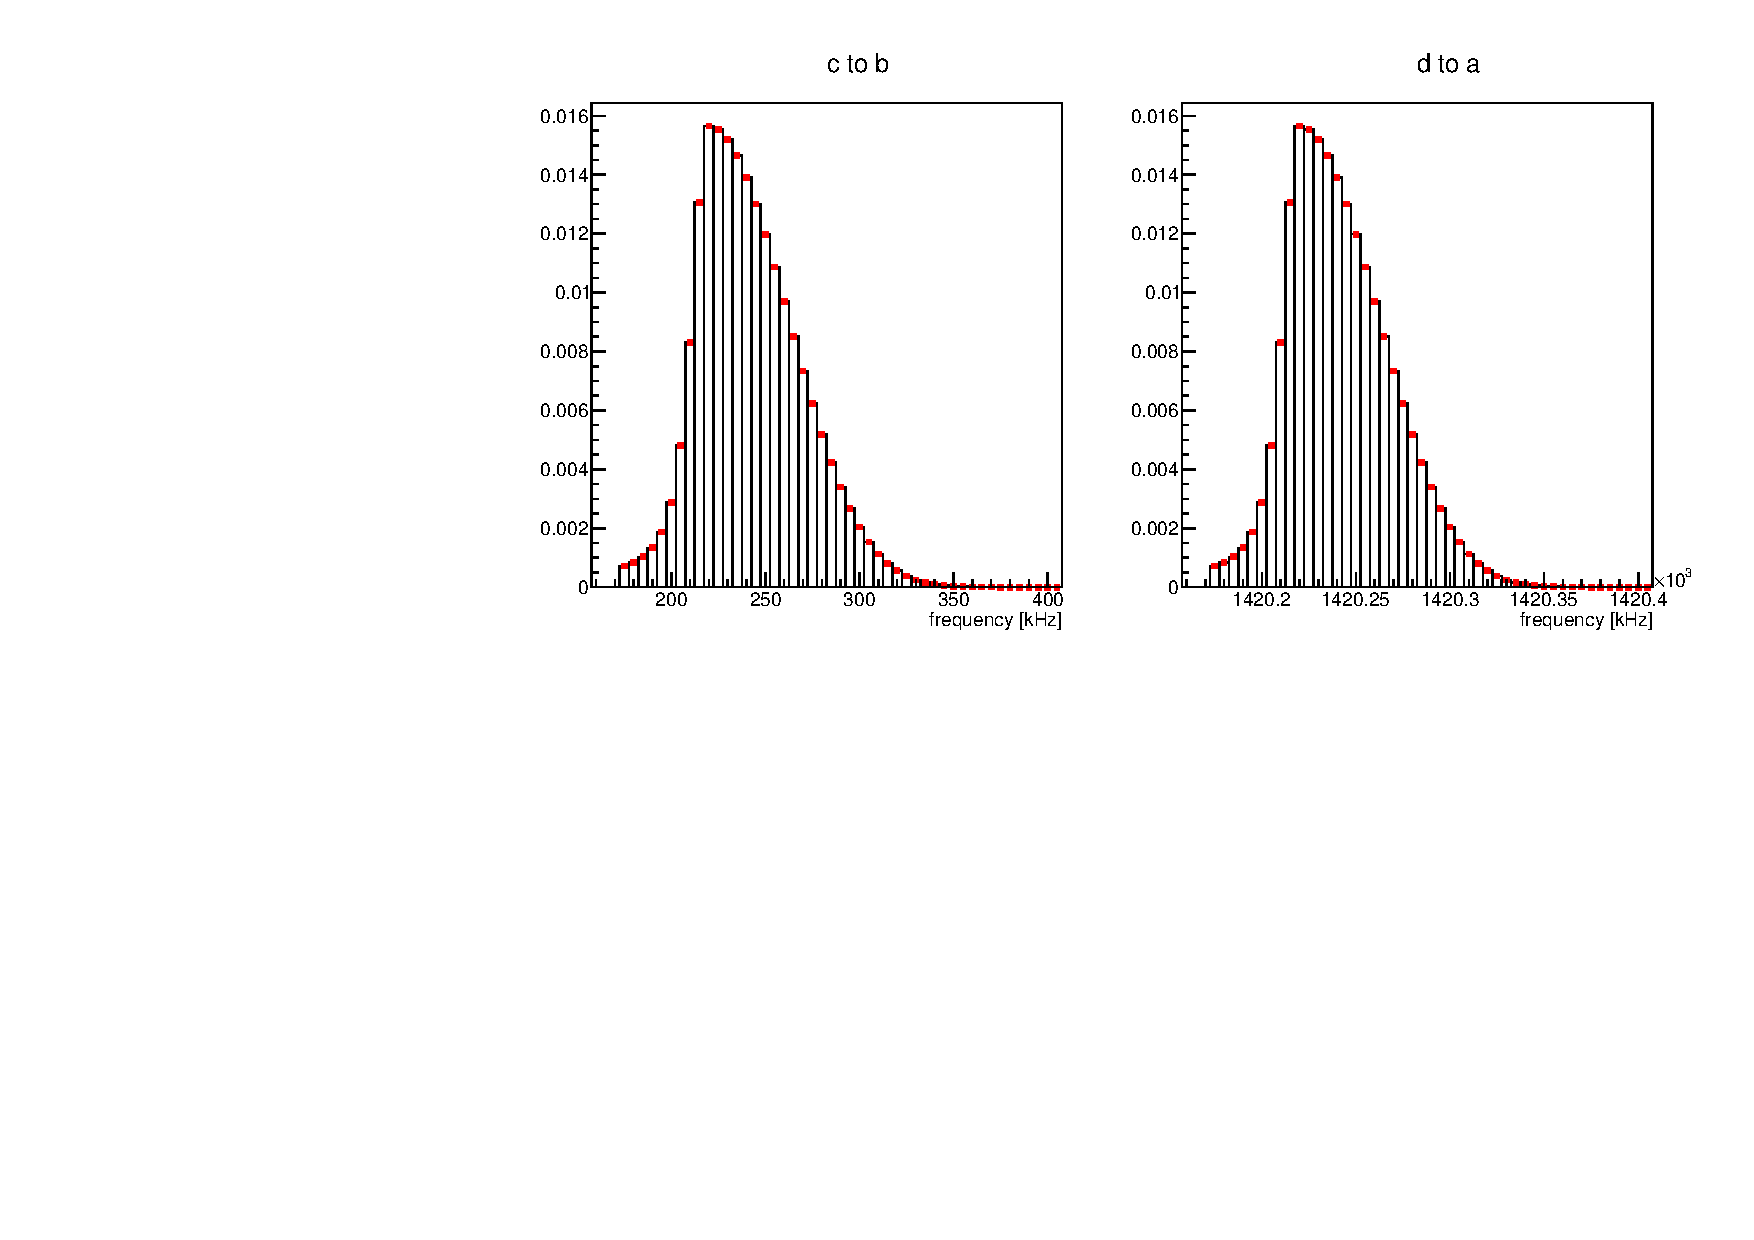
\includegraphics[width = 0.7\textwidth]{../Plot/CruijffLineShapes.pdf}
\end{figure}

The discretized lineshapes here represents the model which the simulation programs uses to generate the data. In blue the lineshape with a $+\SI{2.5}{\kilo \hertz}$ shift, in red the lineshape with a $+\SI{-2.5}{\kilo \hertz}$  with respect to the onset value ( $\SI{0}{\kilo \hertz}$ for c-b and $\SI{1462000}{\kilo \hertz}$ for d-a).
\end{frame}

\begin{frame}{Generate Counts for each frequency}

For illustration purposes, in this plot we show the simulated distribution (24 steps) for a single run with an artificially high number of antihydrogen (5000 in the following plot), without adding the cosmic background:

\begin{figure}[hbtp]
\centering
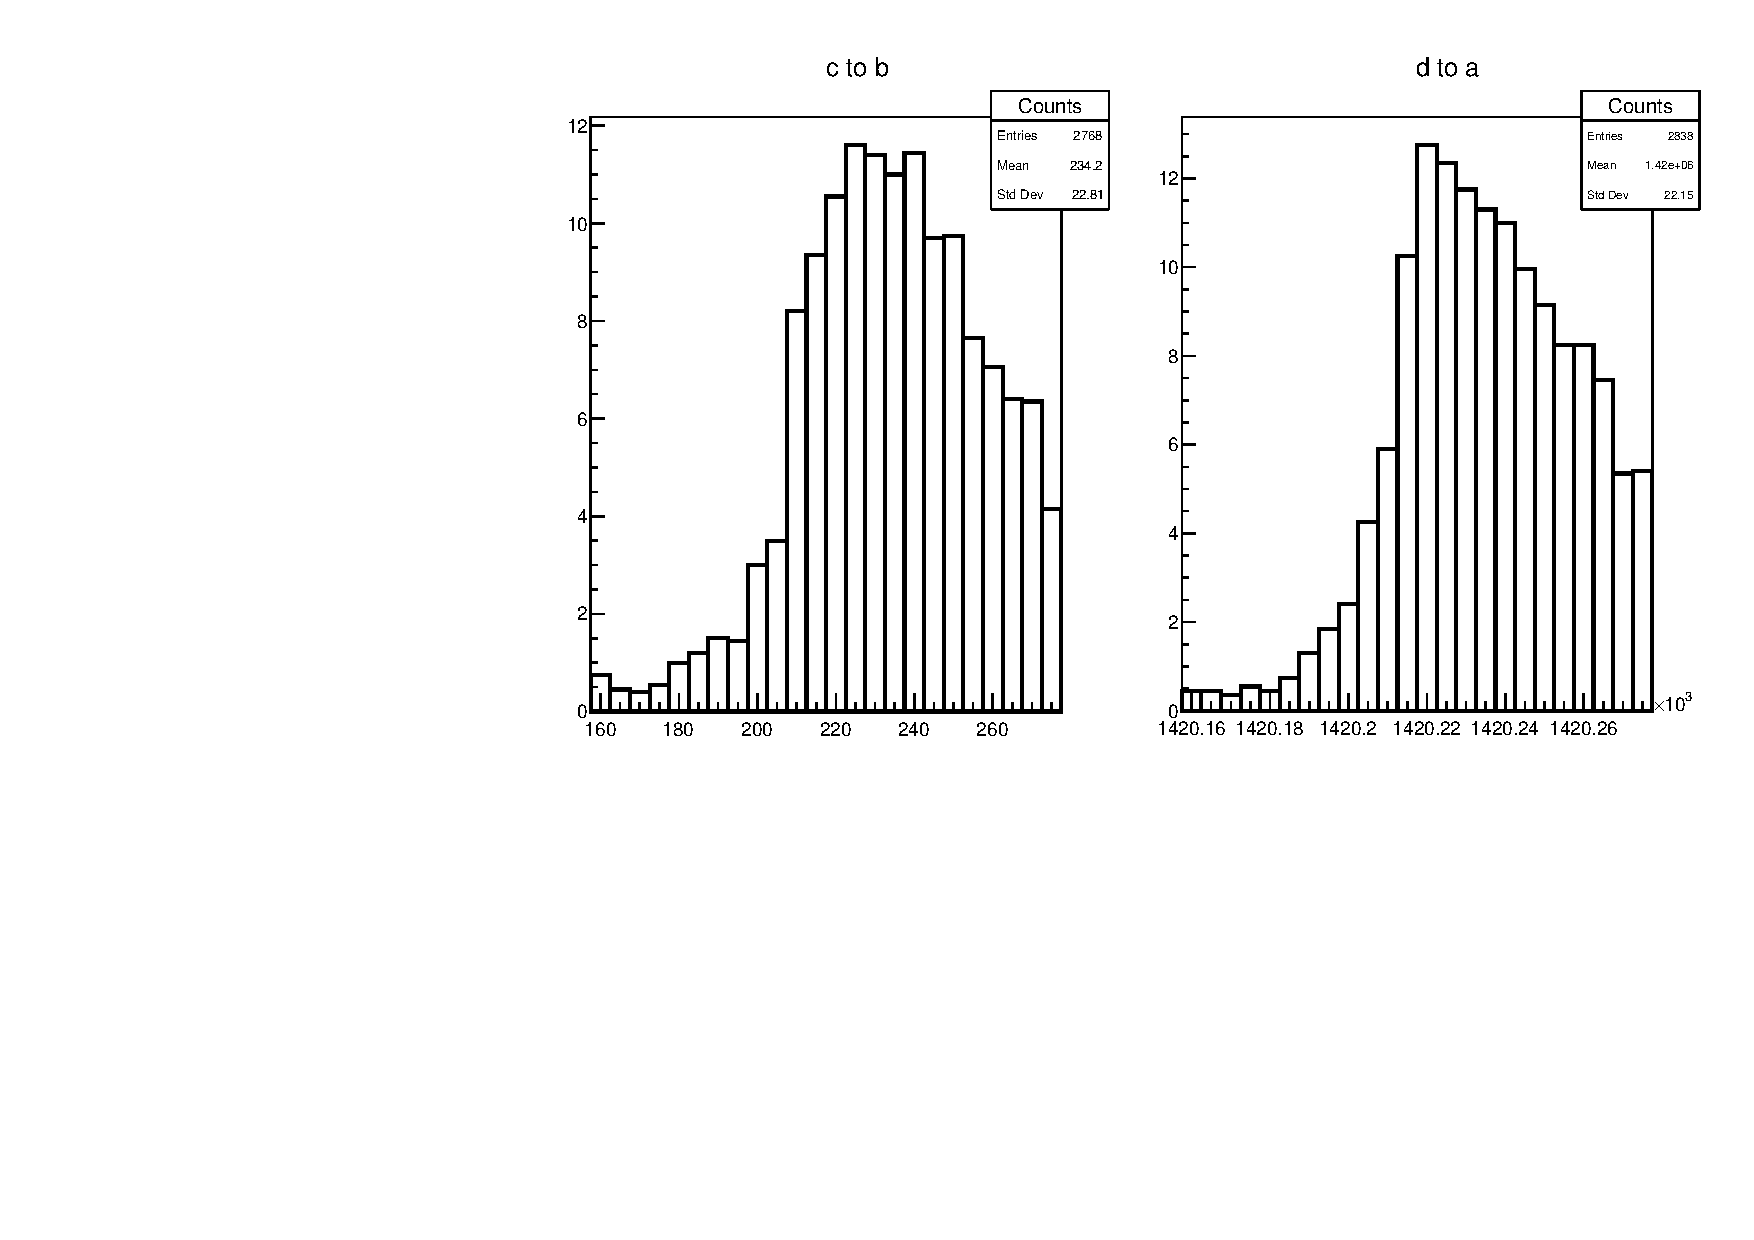
\includegraphics[width = \textwidth]{../Plot/LineshapeSampled.pdf}
%\caption{ Histogram of the generated lineshape.}
\end{figure}
\end{frame}
}

\begin{frame}{Parameters of the Simulation}

We have studies the case of the series of run 4b. The parameters of the simulation are:
\begin{itemize}
\item $N_{stack} = 20$.
\item $N_{\overline{H} \; per \; stack} = 14$.
\item $SweepSteps = 24$.
\item $Repetition = 5$ (not yet used in the following).
\item $TimeStep = \SI{8}{\second}$
\item $FrequencyStep = \SI{5}{\kilo \hertz}$.
\item {\color{red}{$\mu_{cosmic} = \SI{0.051}{\second \tothe{-1}}$
\item $onset_{1, true} = \SI{0}{\kilo \hertz}$ ; $onset_{2, true} = \SI{1420000}{\kilo \hertz}$}}
\item $shift = \pm \SI{2.5}{\kilo \hertz}$.
\end{itemize}

The percentage of events of annihilation to residual gas is set to zero. The amount of anti-hydrogen is divided equally for the two transition c-b and d-a.
\vspace{2pt}
\hrule 
\vspace{2pt}
The first algorithm that we test is the one applied to the data taking of 2017. The onset is exstimated taking the frequence which fulfills the criteria

\begin{equation}
f_{i} : bin(i) > 0; bin(i + 1) > 1
\end{equation}

a second version of the same algorithm is implemented, analyzing the frequencies in decreasing order (reversed algorithm):

\begin{equation*}
f_{i} : bin(i) < 3; bin(i - 1) < 2
\end{equation*}

\end{frame}


\nologo{
\begin{frame}{test 2017 algorithm}

The algorithm is tested for $N_{trial} = 1000$.The amount of events per transition is expected to be poissonian distributed with mean  $\simeq 130$. In this first scenario the cosmic events are removed from the data.

\begin{figure}[hbtp]
\centering
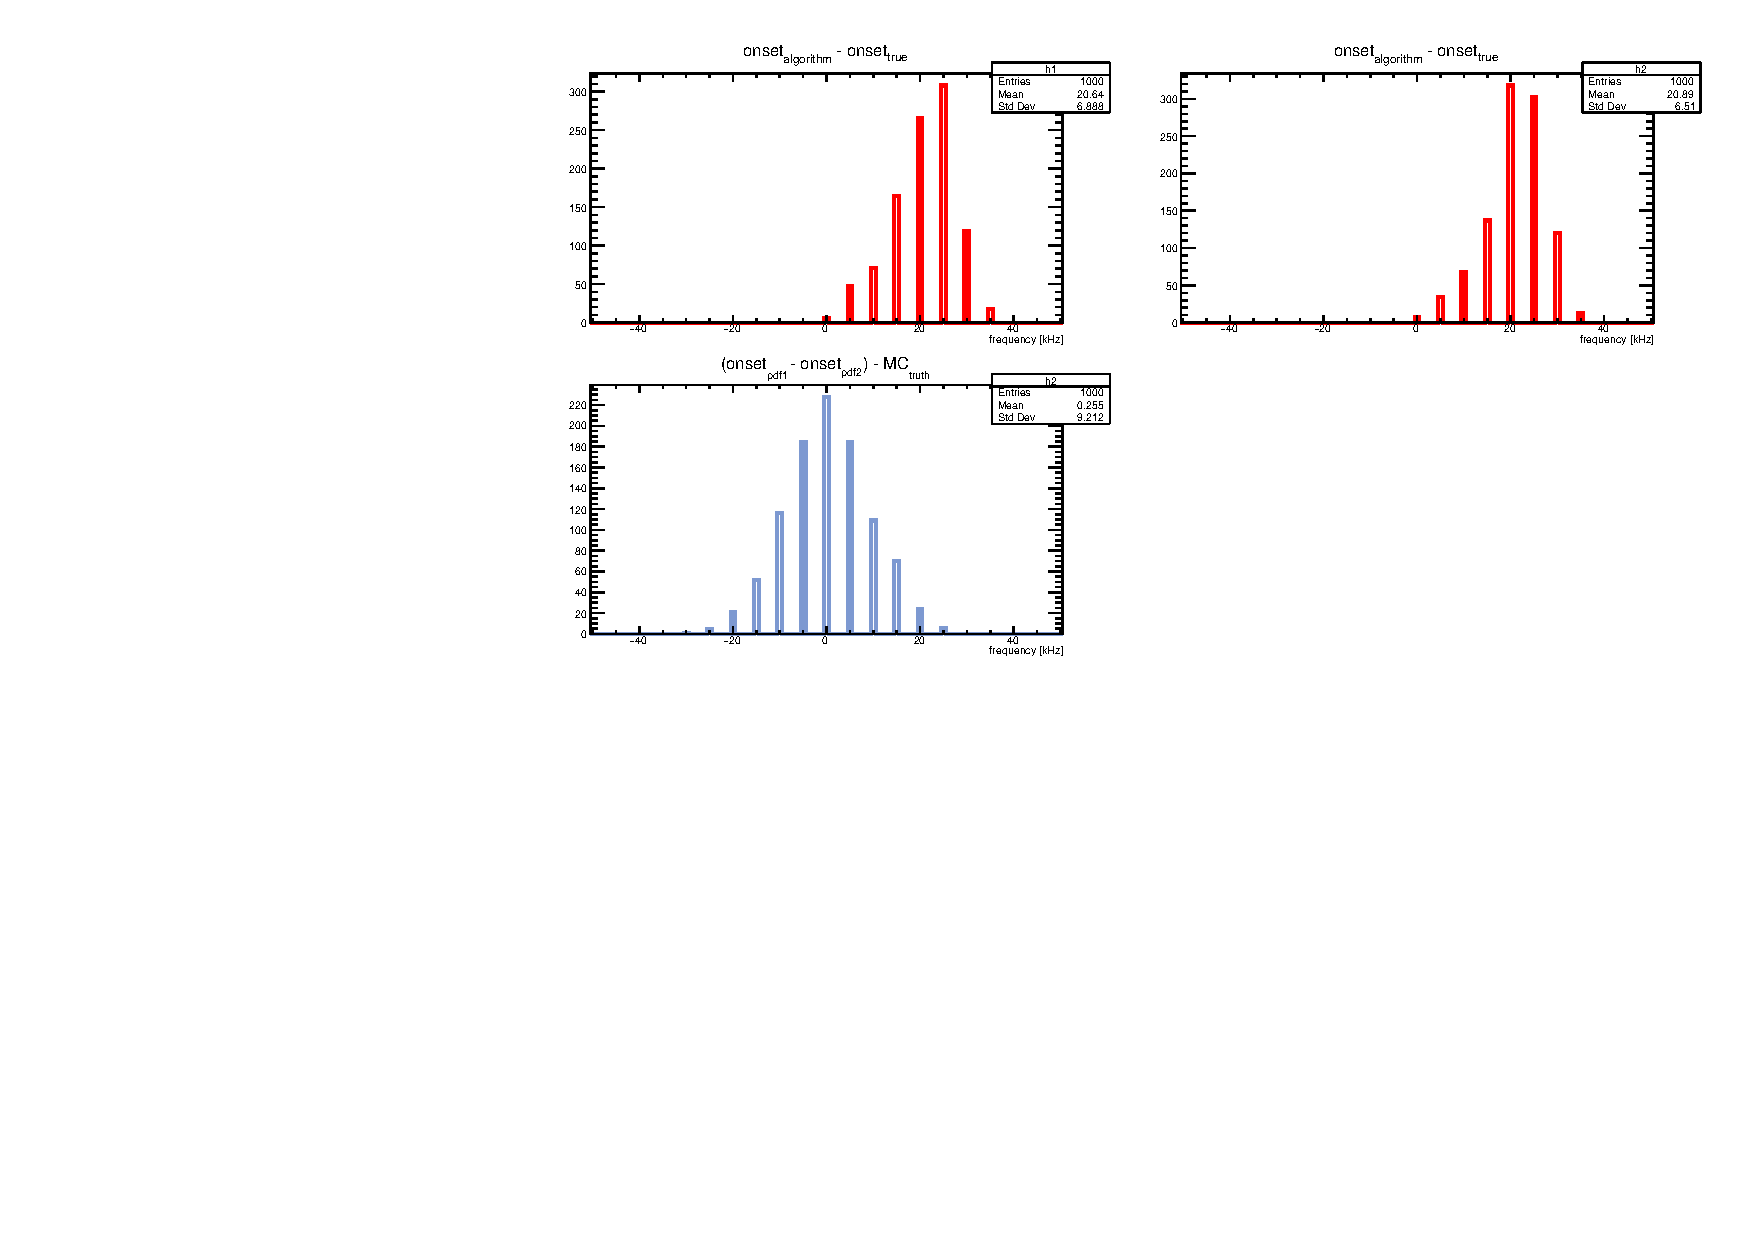
\includegraphics[width = 1\textwidth]{../Plot/2017_foward(cosmic=0).pdf}
\end{figure}
\end{frame}
}

\nologo{
\begin{frame}{test 2017 algorithm}

The algorithm is tested for $N_{trial} = 1000$. The amount of events per transition is expected to be poissonian distributed with mean  $\simeq 130$. The cosmic background is fixed to $0.41$ events per frequence.

\begin{figure}[hbtp]
\centering
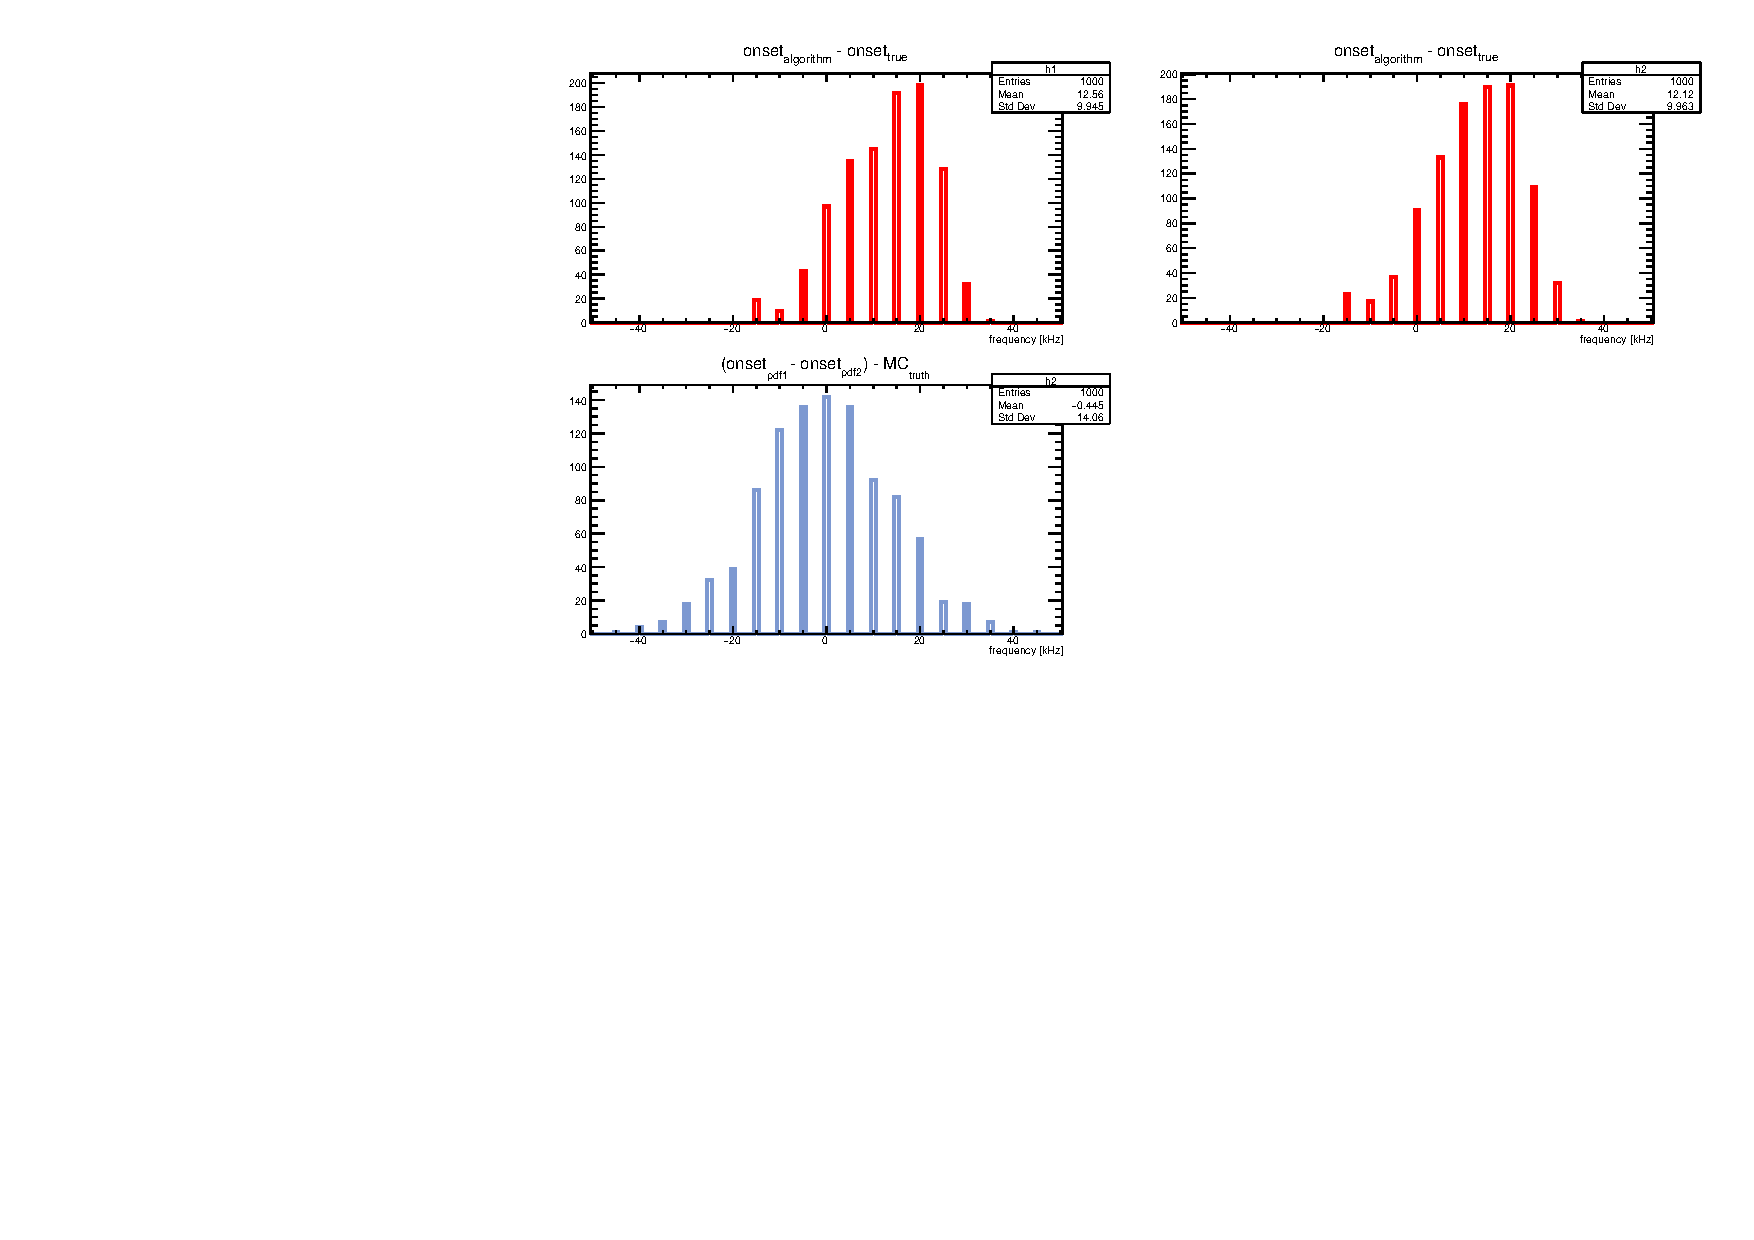
\includegraphics[width = 1\textwidth]{../Plot/2017_foward.pdf}
\end{figure}
\end{frame}
}

\nologo{
\begin{frame}{test 2017 algorithm (reversed)}

The algorithm is tested for $N_{trial} = 1000$. The amount of events per transition is expected to be poissonian distributed with mean  $\simeq 130$. In this scenario the cosmic background is removed.

\begin{figure}[hbtp]
\centering
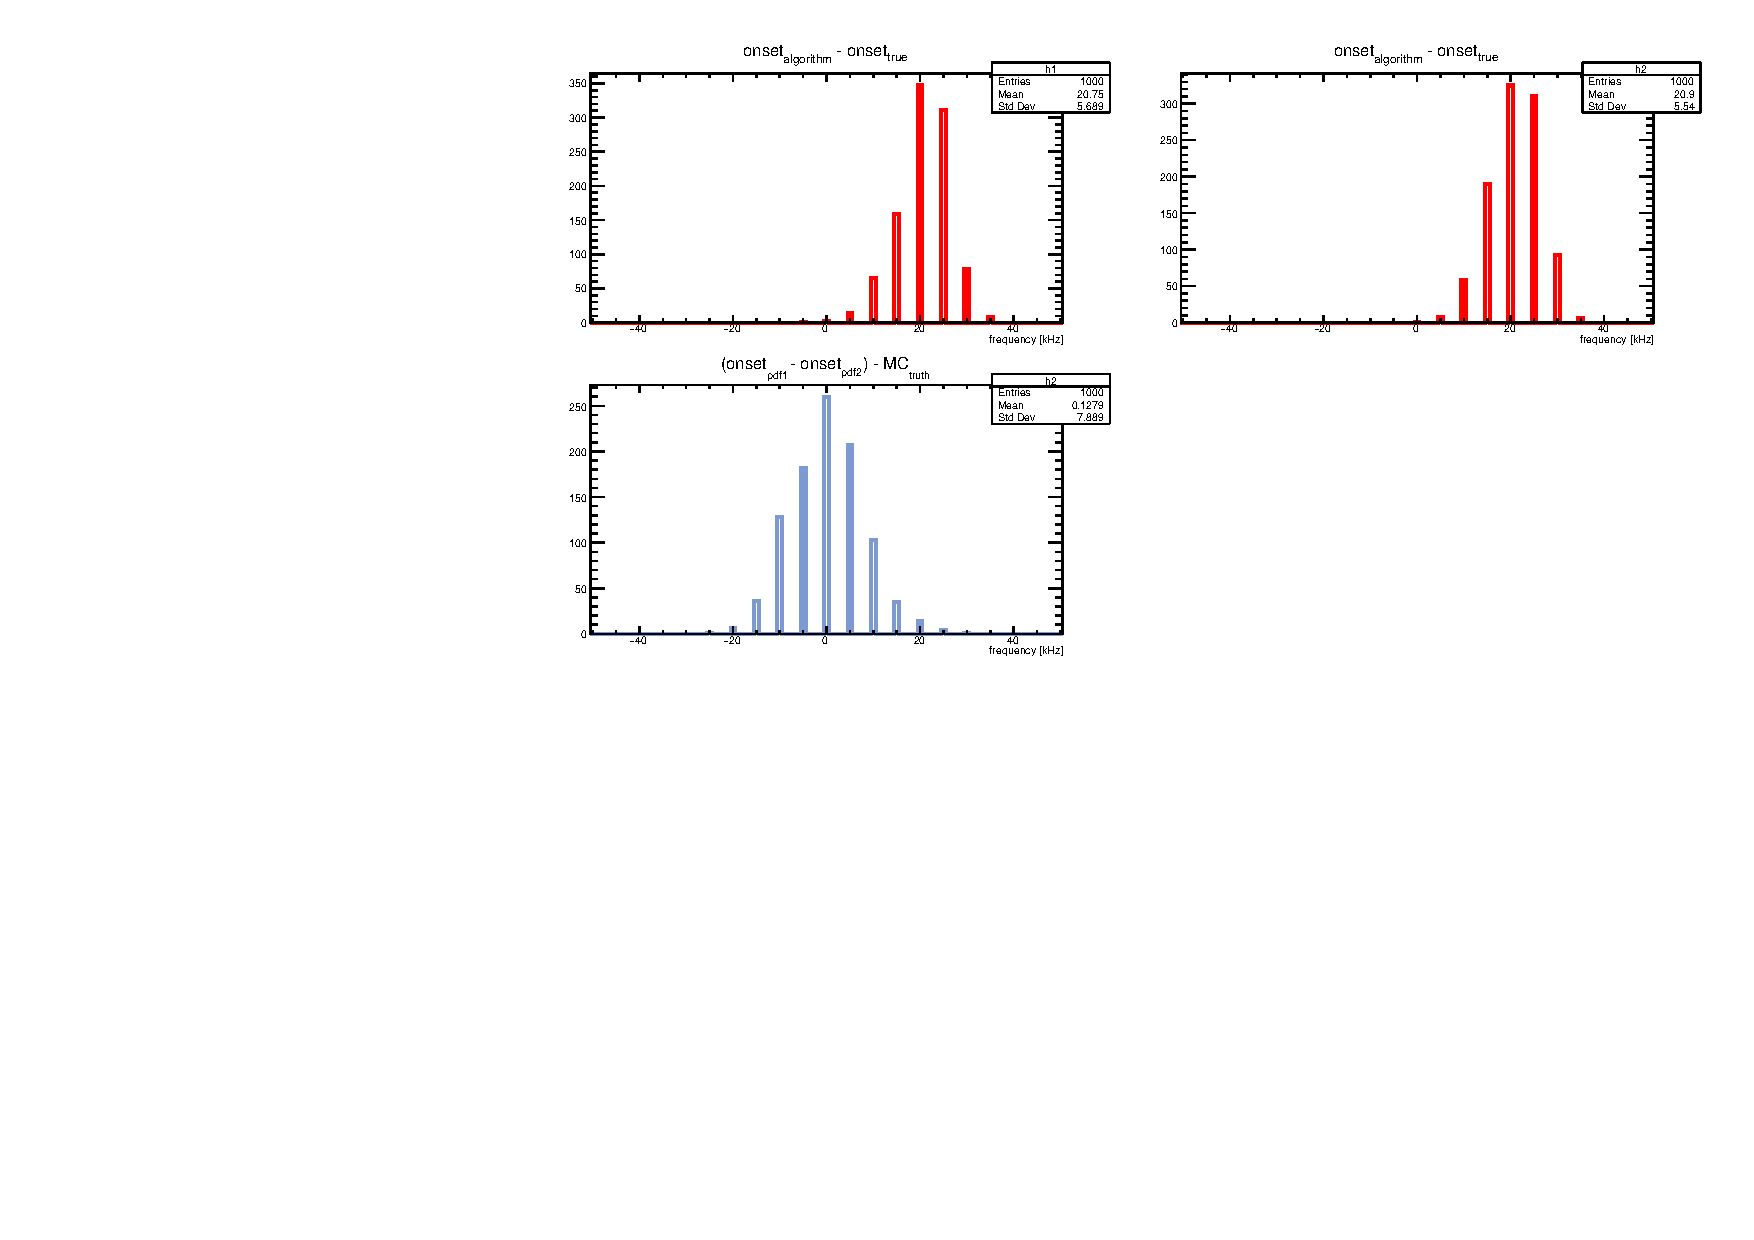
\includegraphics[width = 1\textwidth]{../Plot/2017_reversed(cosmic=0).pdf}
\end{figure}
\end{frame}
}

\nologo{
\begin{frame}{test 2017 algorithm (reversed)}

The algorithm is tested for $N_{trial} = 1000$. The amount of events per transition is expected to be poissonian distributed with mean  $\simeq 130$. The cosmic background is fixed to $0.41$ events per frequence. 

\begin{figure}[hbtp]
\centering
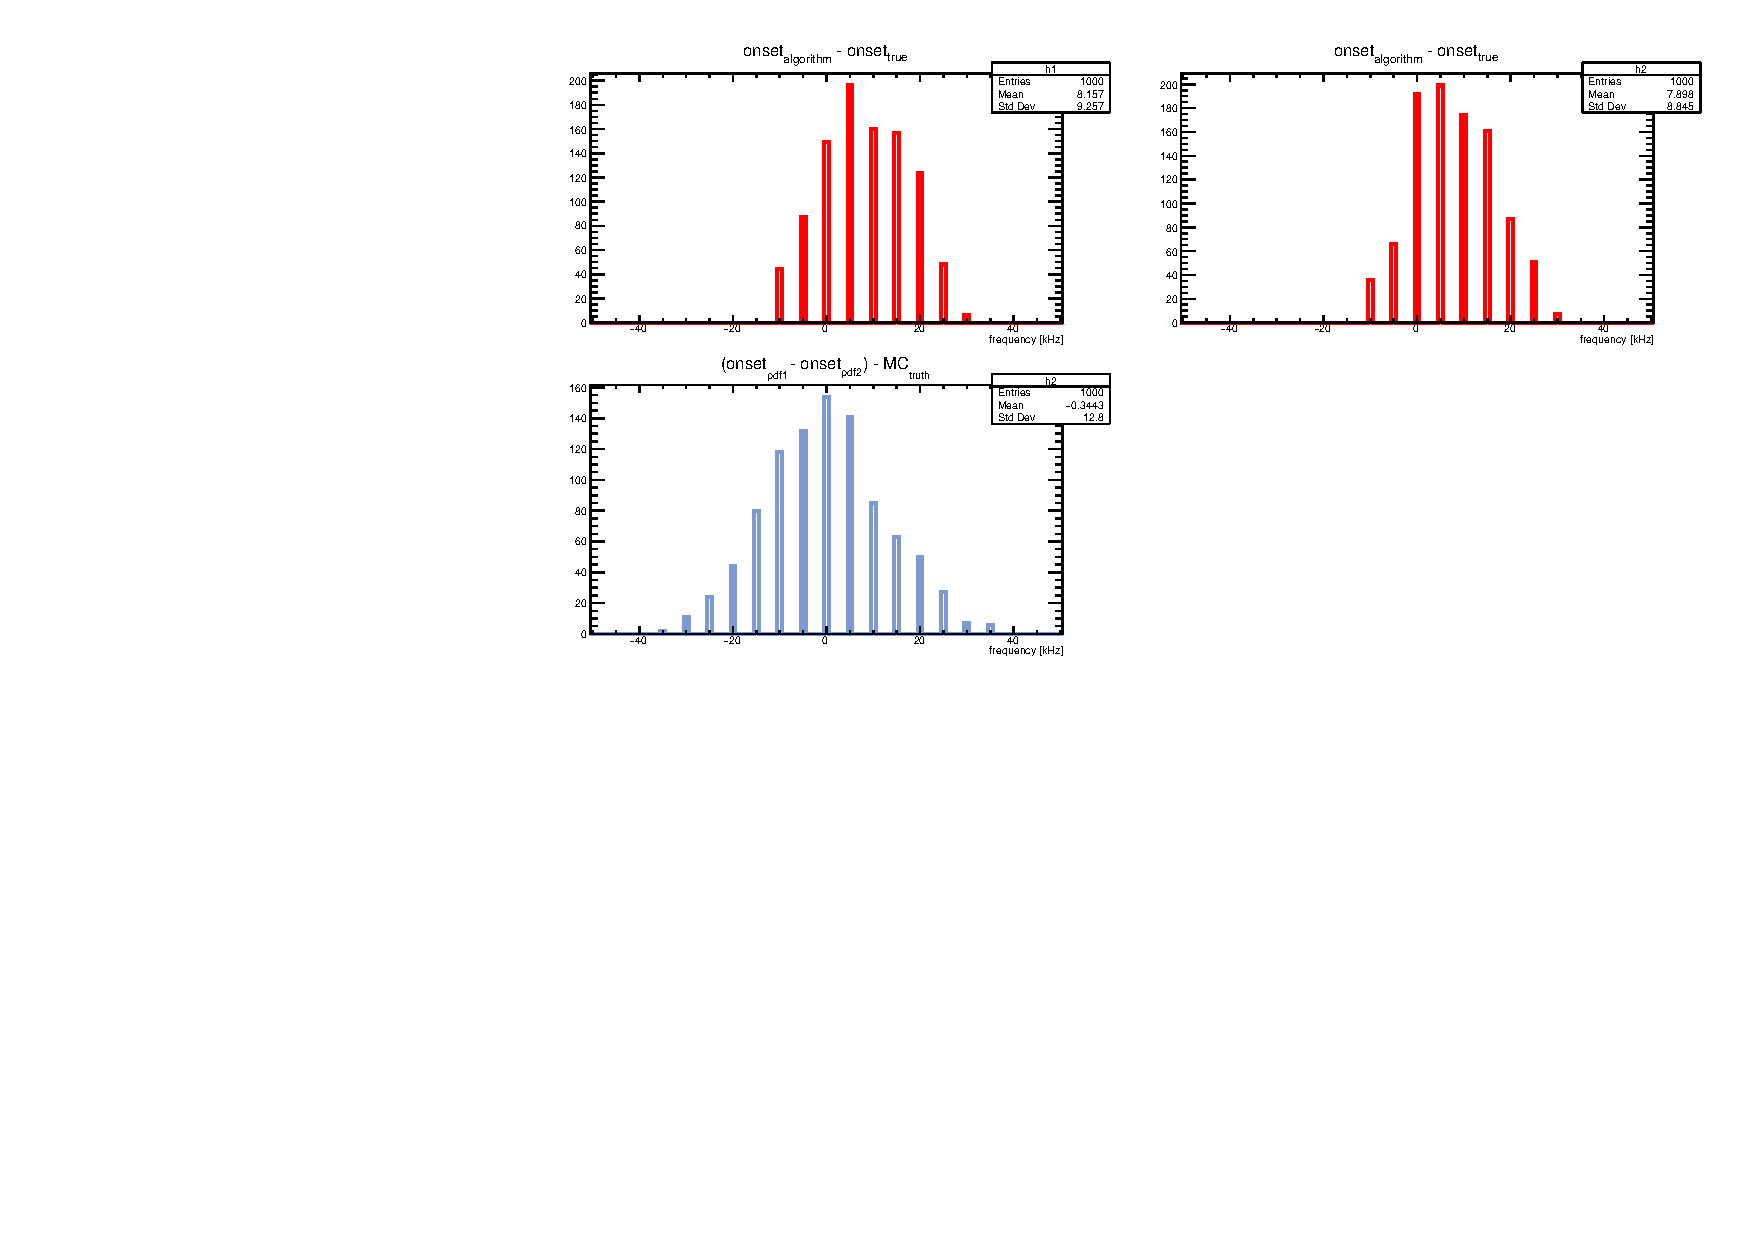
\includegraphics[width = 1\textwidth]{../Plot/2017_reversed.pdf}
\end{figure}
\end{frame}
}

\begin{frame}{Other stategies}

We have tested other 2 different algorithms, that can be useful to identify the onset. The first algorithm indetifies the onset ad the first frequency with counts over threshold:

\begin{equation}
f_{i} : bin_{i} > Threshold
\end{equation}

The second algorithms is a constant fraction discriminator. It works similarly to the previous algorithm, except for the fact that the threshold is computed each time as:

\begin{equation}
threshold = p \cdot max\{bin_{i}  \}
\end{equation}

where $p$ is a parameter of the algorithm, in the range (0,1).

In the end we have tested another algorithm (\textit{sumNeighbors}), defined is this way:
\begin{equation}
f_{i} : bin_{i} + bin_{i+1} + bin_{i +2} > 3\cdot \mu_{cosmic} + \sqrt{3}   N \cdot \sqrt{\mu_{cosmic}} 
\end{equation}

Where $N$ is a parameter of the algorithm. This algorithm is directly derived from the t-student test.

\end{frame}

\begin{frame}{Results}

\begin{table}
\center
\resizebox{\textwidth}{!}{
\begin{tabular}{l|l l l l l}
\hline 
algorithms & $\mu$ $[\SI{}{\kilo \hertz}]$  
		   & $\sigma$  $[\SI{}{\kilo \hertz}]$
		   & $\mu$ $[\SI{}{\kilo \hertz}]$
		   & $\sigma$ $[\SI{}{\kilo \hertz}]$ \\ 
\hline
 						 	  &  \multicolumn{2}{c}{\color{blue}{without cosmic background}}     & \multicolumn{3}{c}{\color{blue}{with cosmic background}}  \\
\hline
2017 ($ > 0 ; > 1$ )          & $-0.18$  & $9.7$   & $-0.445$ & $14.1$\\ 

2017 reversed ($ < 2; < 1$)   & $+0.13$ & $7.89$   & $+0.25$  & $9.73$\\ 

threshold ($ > 1$)            & $+0.025$ & $11.5$  & $+0.005$ & $16.72$\\ 

threshold ($ > 2$)            & $-0.06$  & $9.56$  & $+0.67$  & $14.1$\\ 

threshold ($ > 3$)            & $-0.1$   & $7.48$  & $-0.07$  & $9.96$ \\

const. fraction ($ p = 10 \% $) & $-0.02$  & $11.56$ & $+0.19$   & $16.66$\\ 
 
const. fraction ($ p = 20 \% $) & $-0.215$ & $9.05$  & $+0.55$   & $13.06$\\ 

const. fraction ($ p = 30 \% $) & $+0.08$  & $7.43$  & $+0.05$   & $8.84$ \\

sumNeighbors ($ N = 1 $) & $+0.01$  & $9.47$  & $+0.055$   & $13.03$ \\

sumNeighbors ($ N = 2 $) & $-0.425$  & $8.83$  & $+0.005$   & $12.69$ \\

sumNeighbors ($ N = 3 $) & $-0.47$  & $7.85$  & $+0.115$   & $11.66$ \\
\hline
\end{tabular}}
\caption{ Result of the simulation for $N_{trials} = 1000$. In the first two column the cosmic background is removed from the data. The last two columns contains the result of the simulation adding the cosmic background. The $\mu$ and $\sigma$ are the quantities computed from the distribution of $(onset_{2} - onset_{1}) - MC_{truth}$.}
\end{table}
\end{frame}

\begin{frame}

\begin{figure}
\centering
\subfloat[][\emph{algorithm 2017}]
{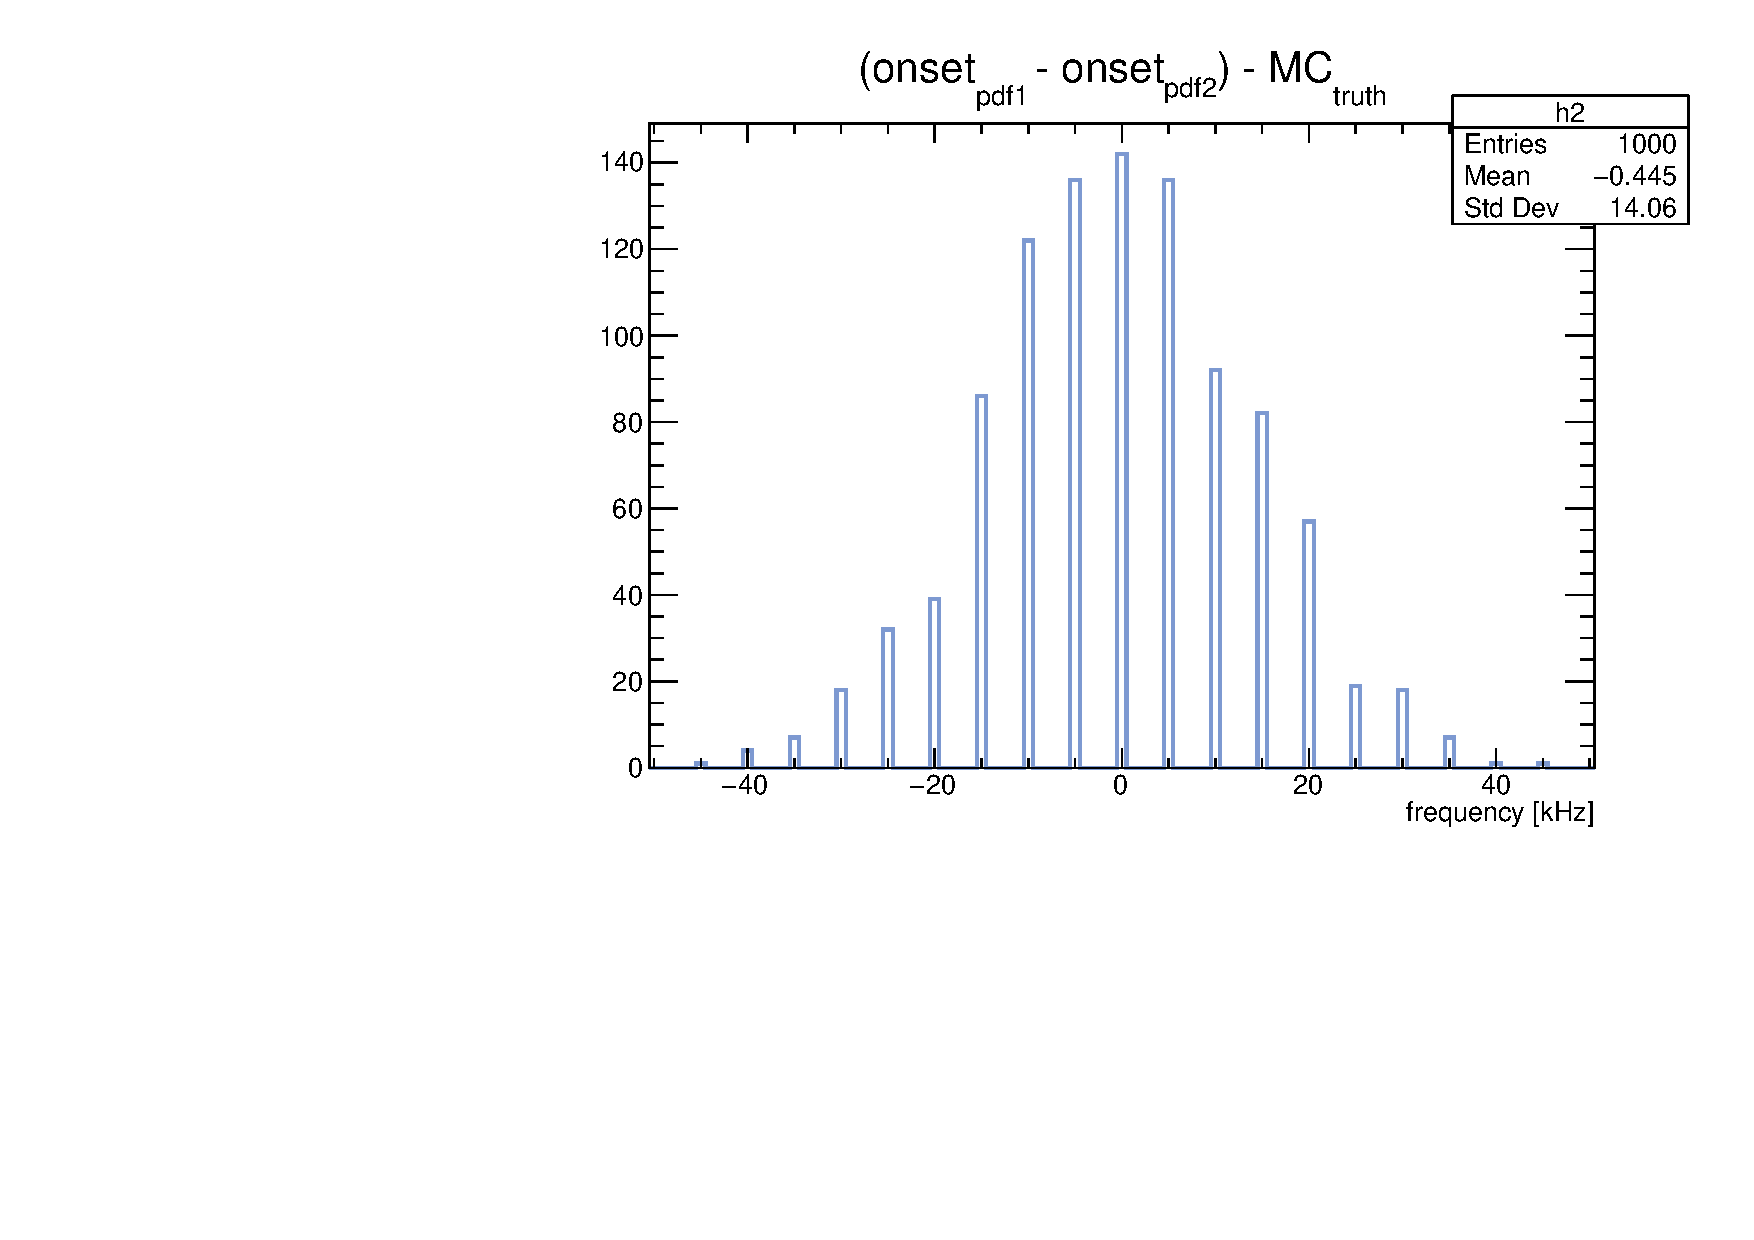
\includegraphics[width=.30\textwidth]{../Plot/delta_2017_foward.pdf}} 
\subfloat[][\emph{algorithm 2017 reversed}]
{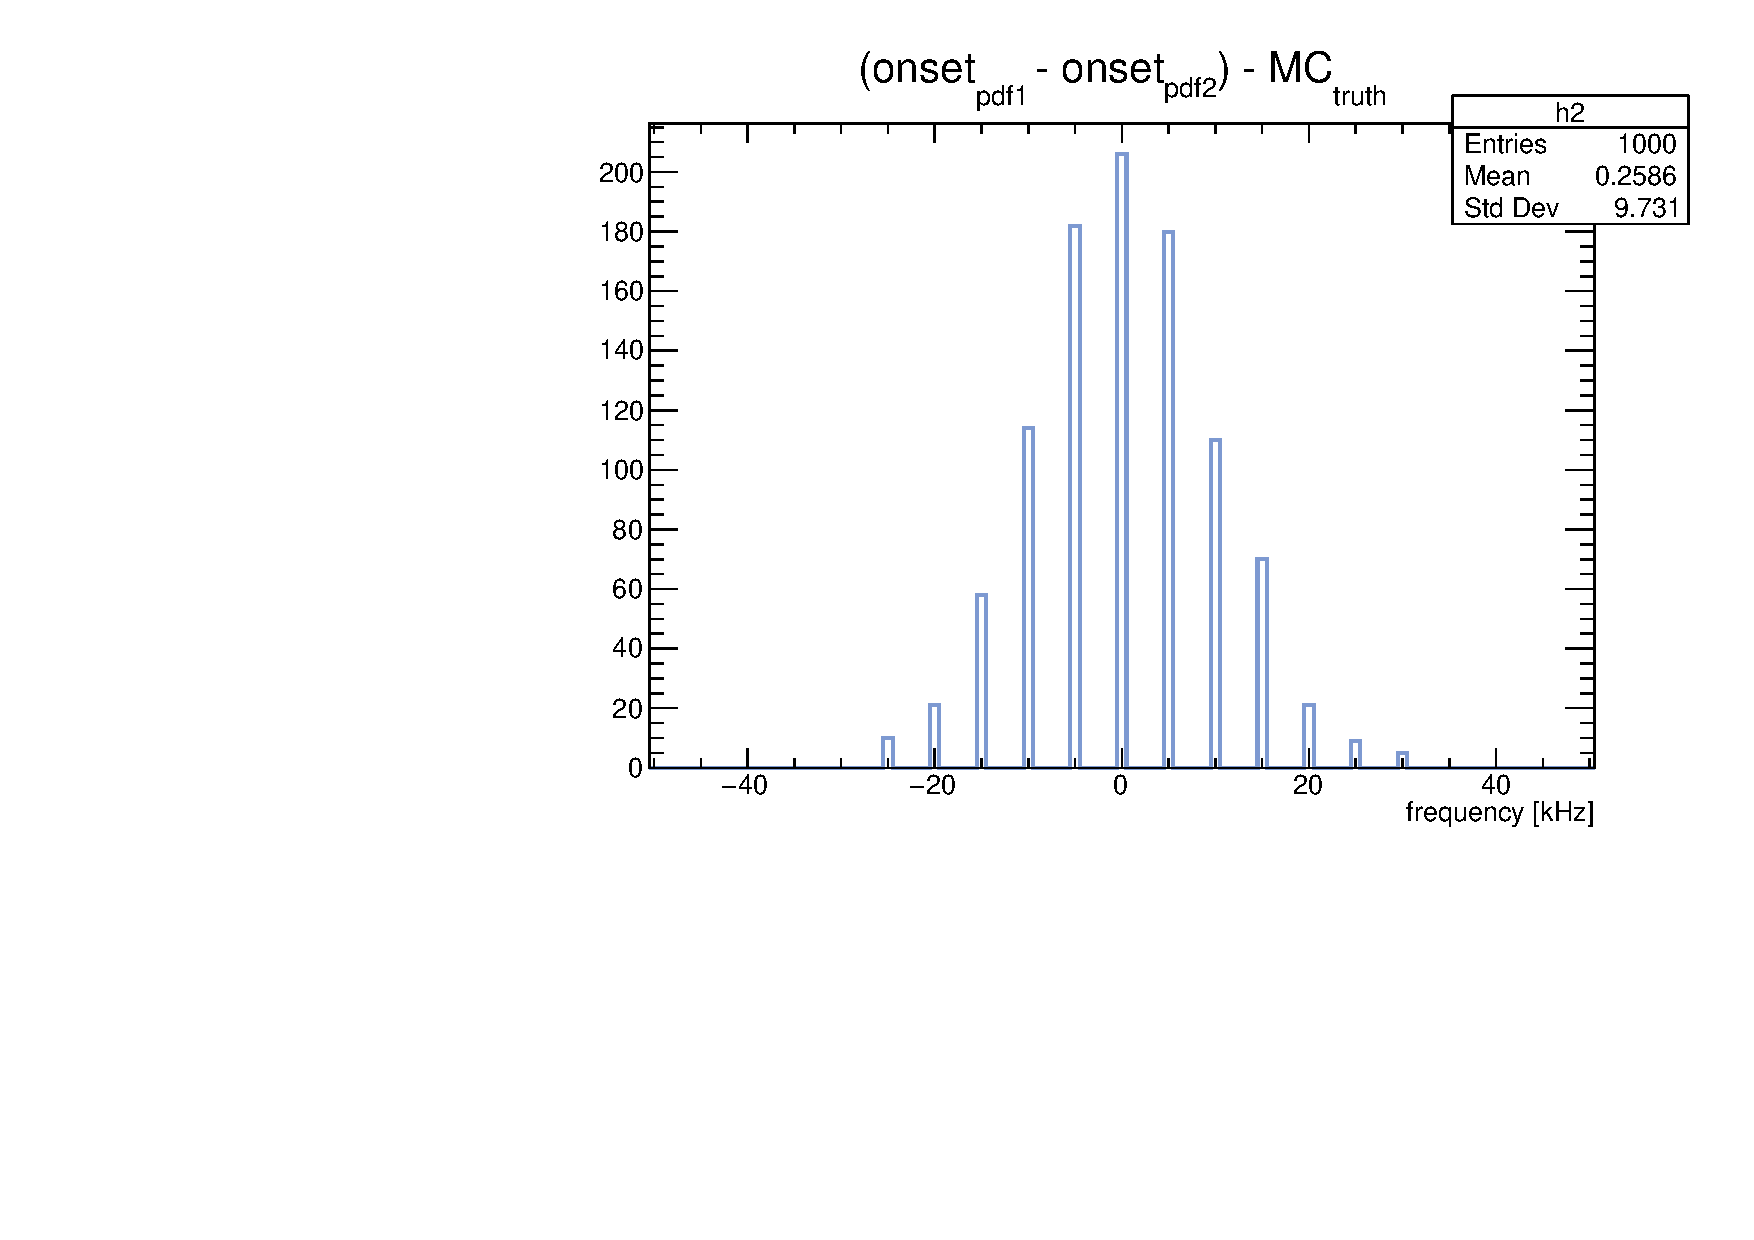
\includegraphics[width=.30\textwidth]{../Plot/delta_2017_reversed.pdf}} 
\subfloat[][\emph{threshold ($> 2$)}]
{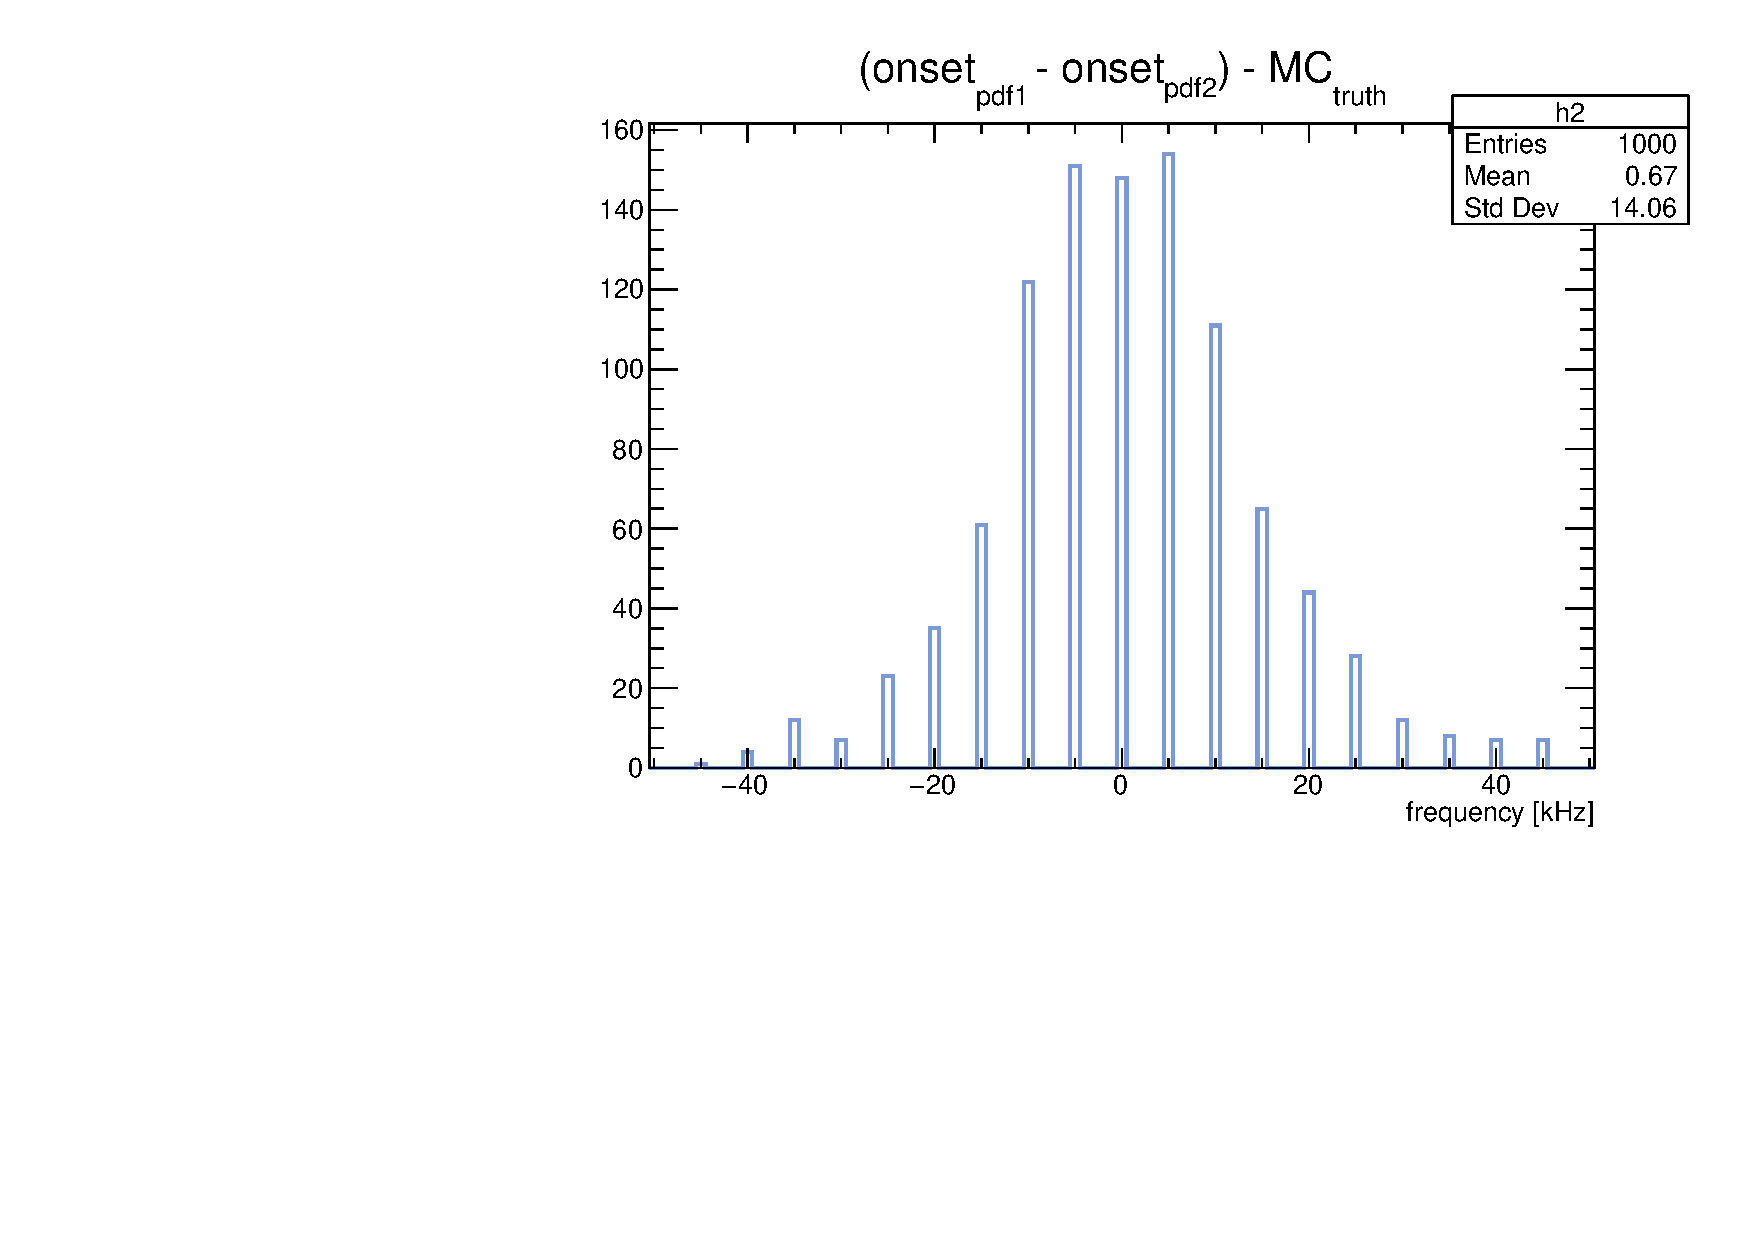
\includegraphics[width=.30\textwidth]{../Plot/delta_Threshold_2.pdf}} \\
\subfloat[][\emph{threshold ($> 3$)}]
{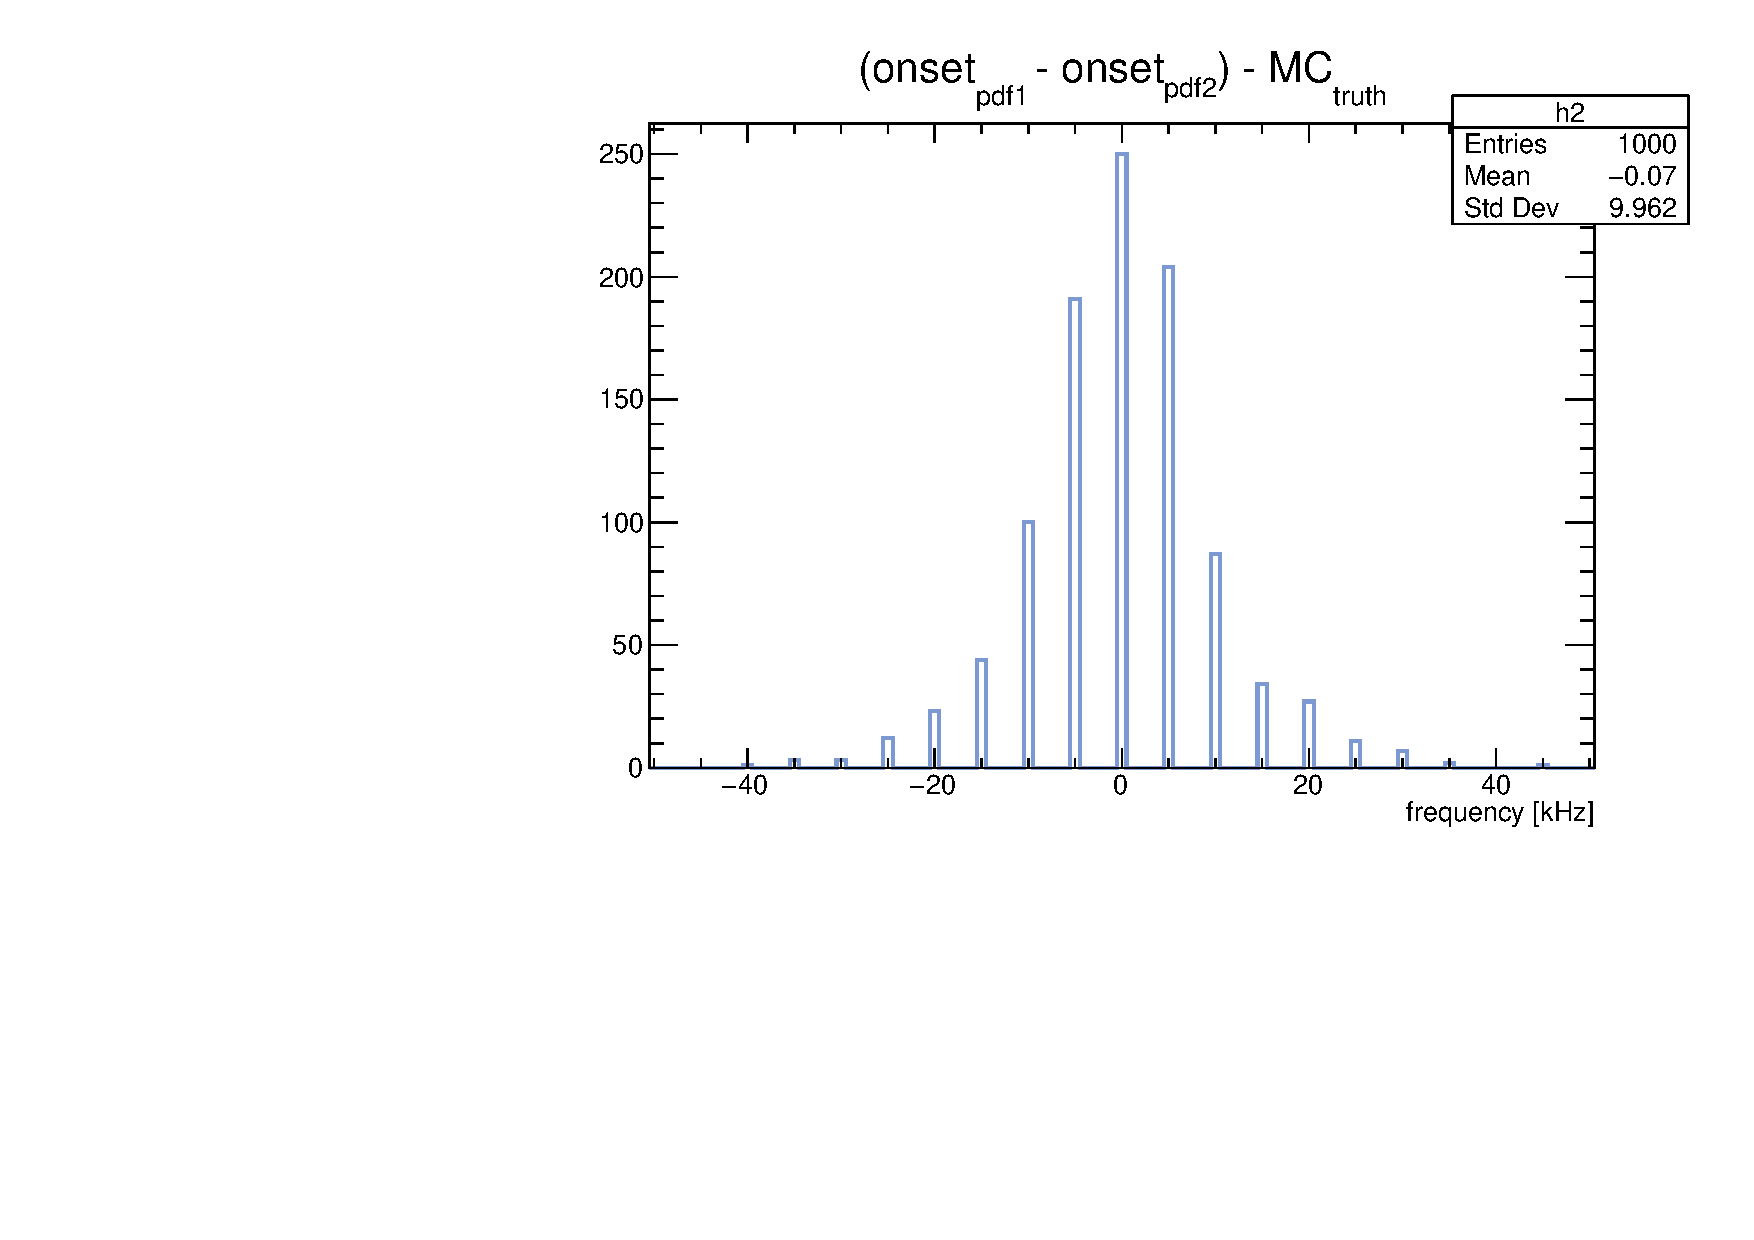
\includegraphics[width=.30\textwidth]{../Plot/delta_Threshold_3.pdf}}
\subfloat[][\emph{const fraction ($> 20\%$)}]
{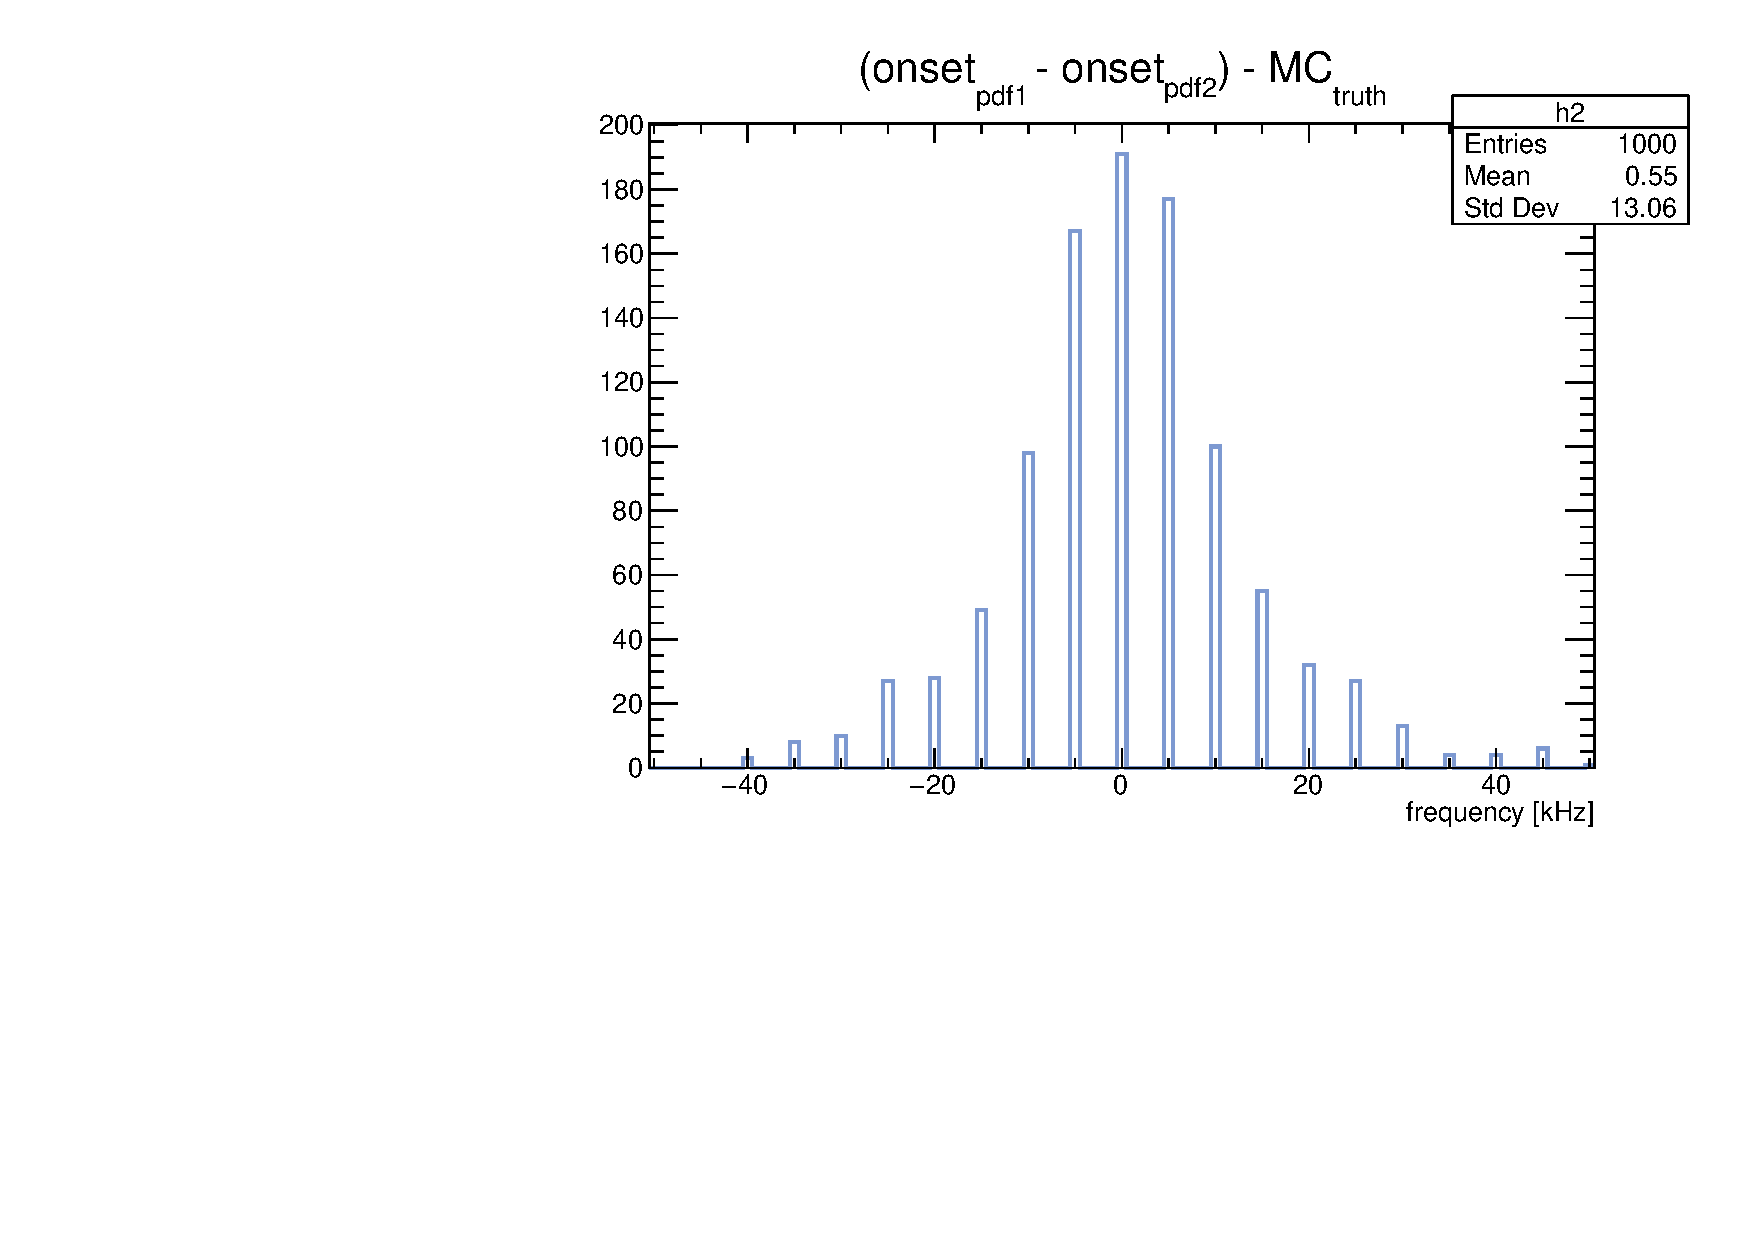
\includegraphics[width=.30\textwidth]{../Plot/delta_constFract_20.pdf}} 
\subfloat[][\emph{const fraction ($> 30\%$)}]
{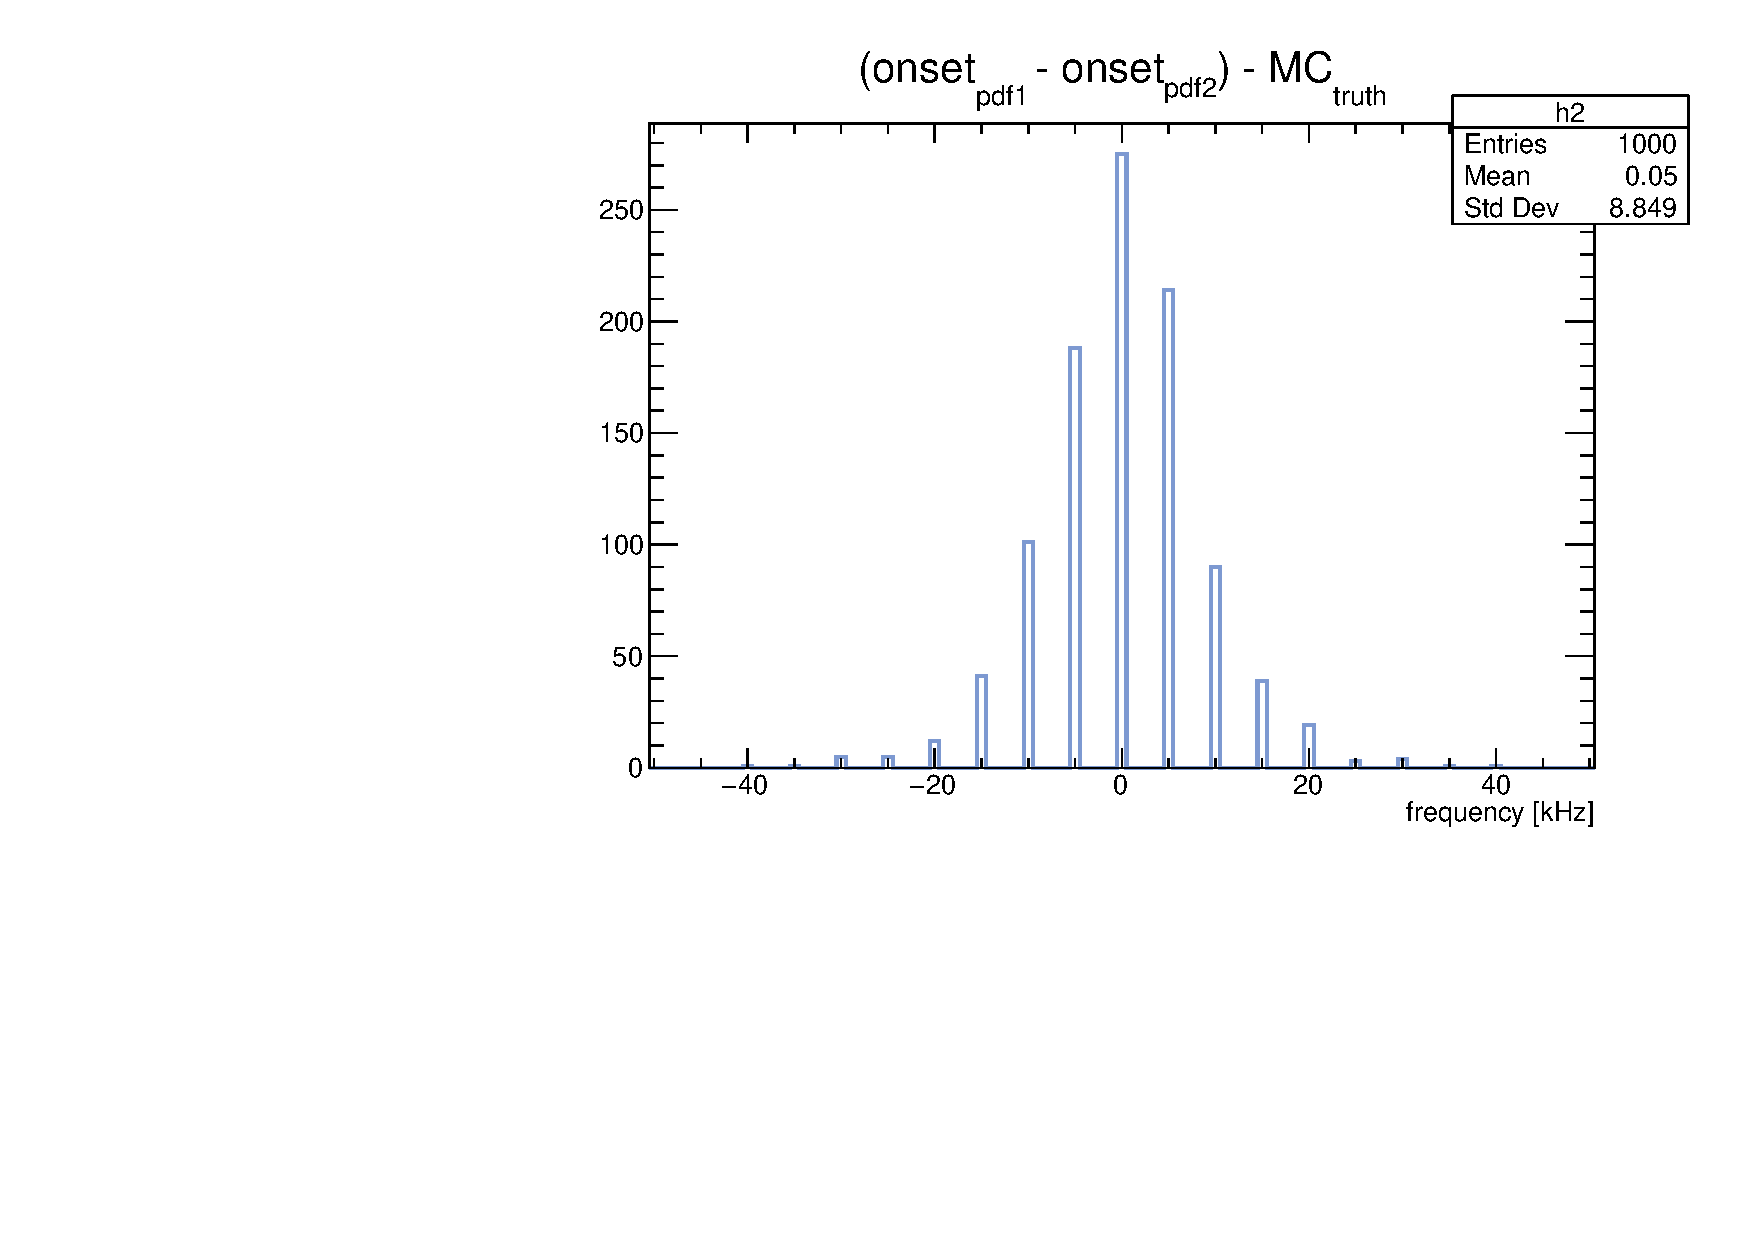
\includegraphics[width=.30\textwidth]{../Plot/delta_constFract_30.pdf}}
\end{figure}
\end{frame}

\begin{frame}
\begin{figure}
\centering
\subfloat[][\emph{sumNeighbors ($N > 2$)}]
{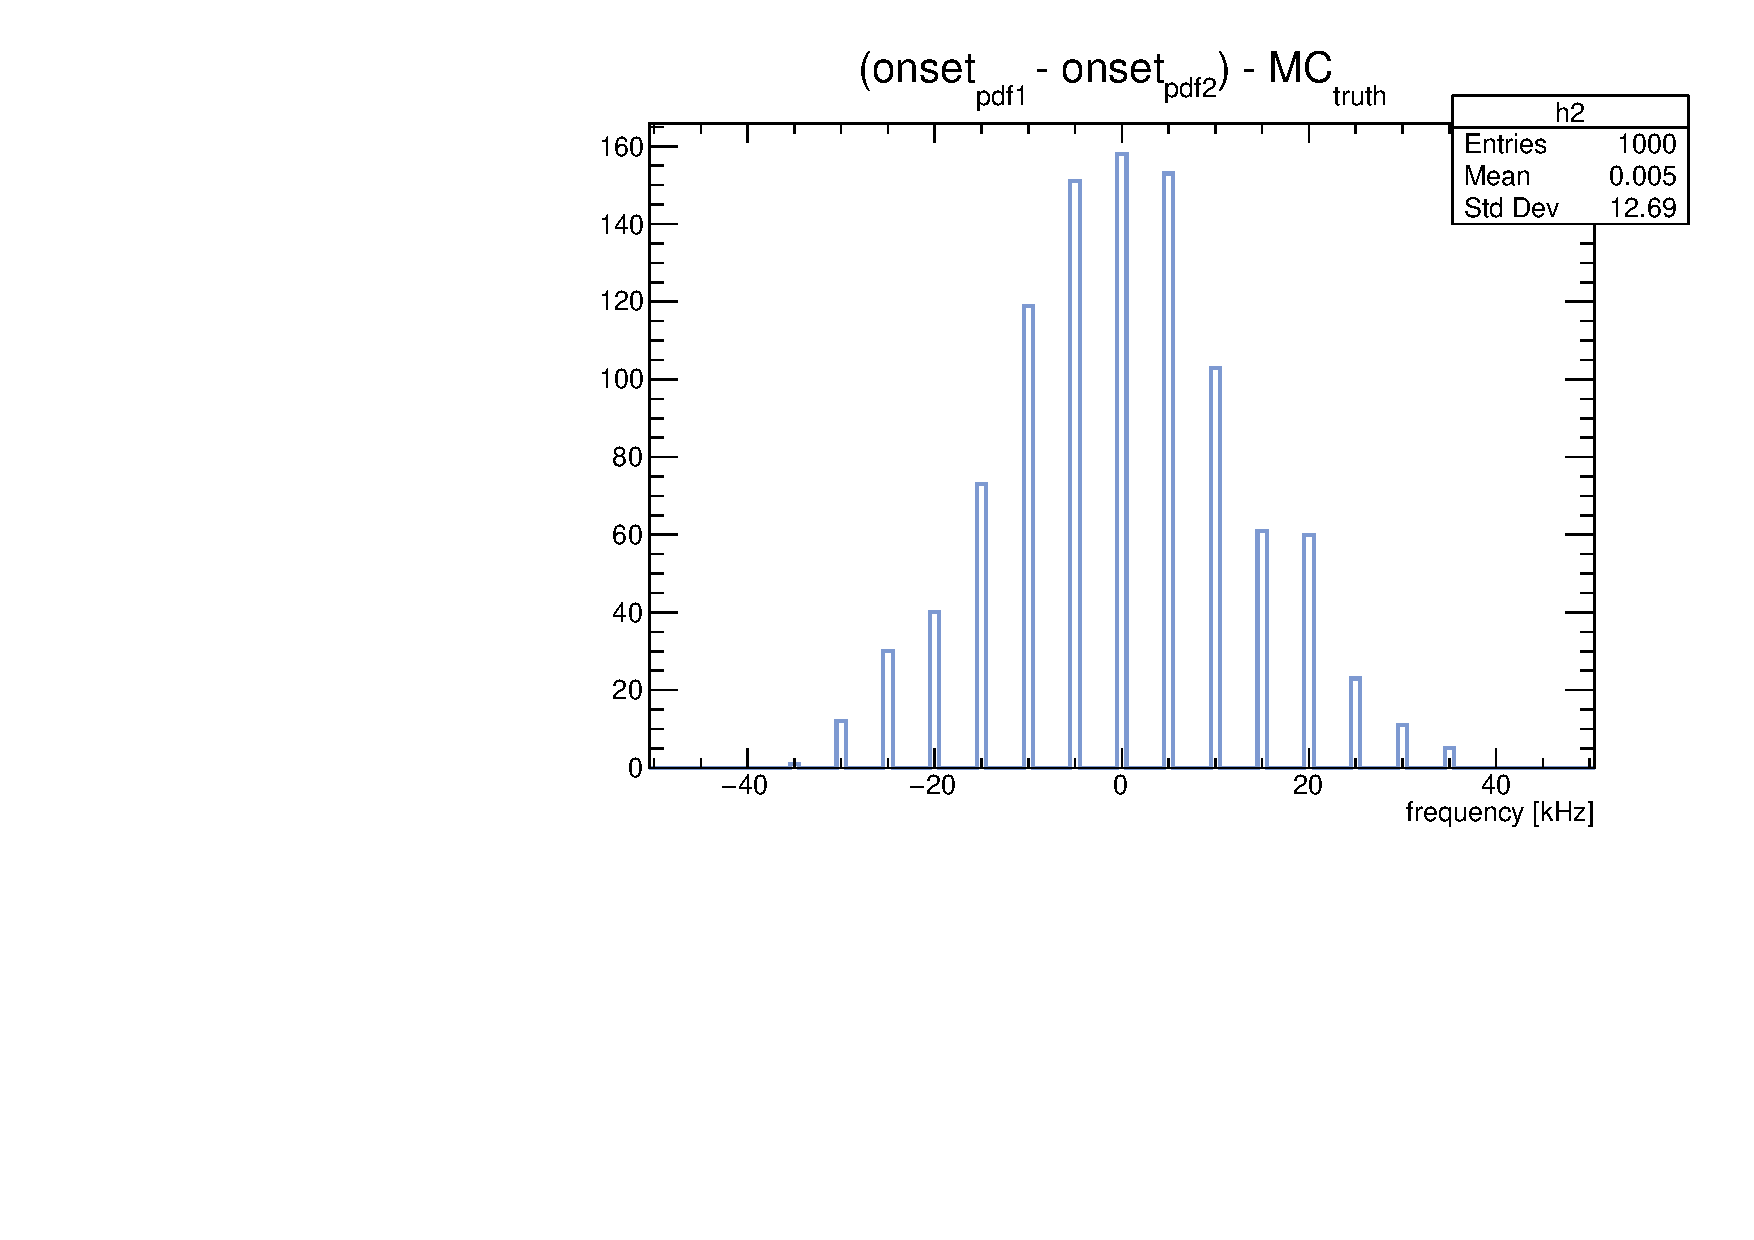
\includegraphics[width=.45\textwidth]{../Plot/delta_sumNeighbors_sigma20.pdf}}
\subfloat[][\emph{sumNeighbors ($N > 3$)}]
{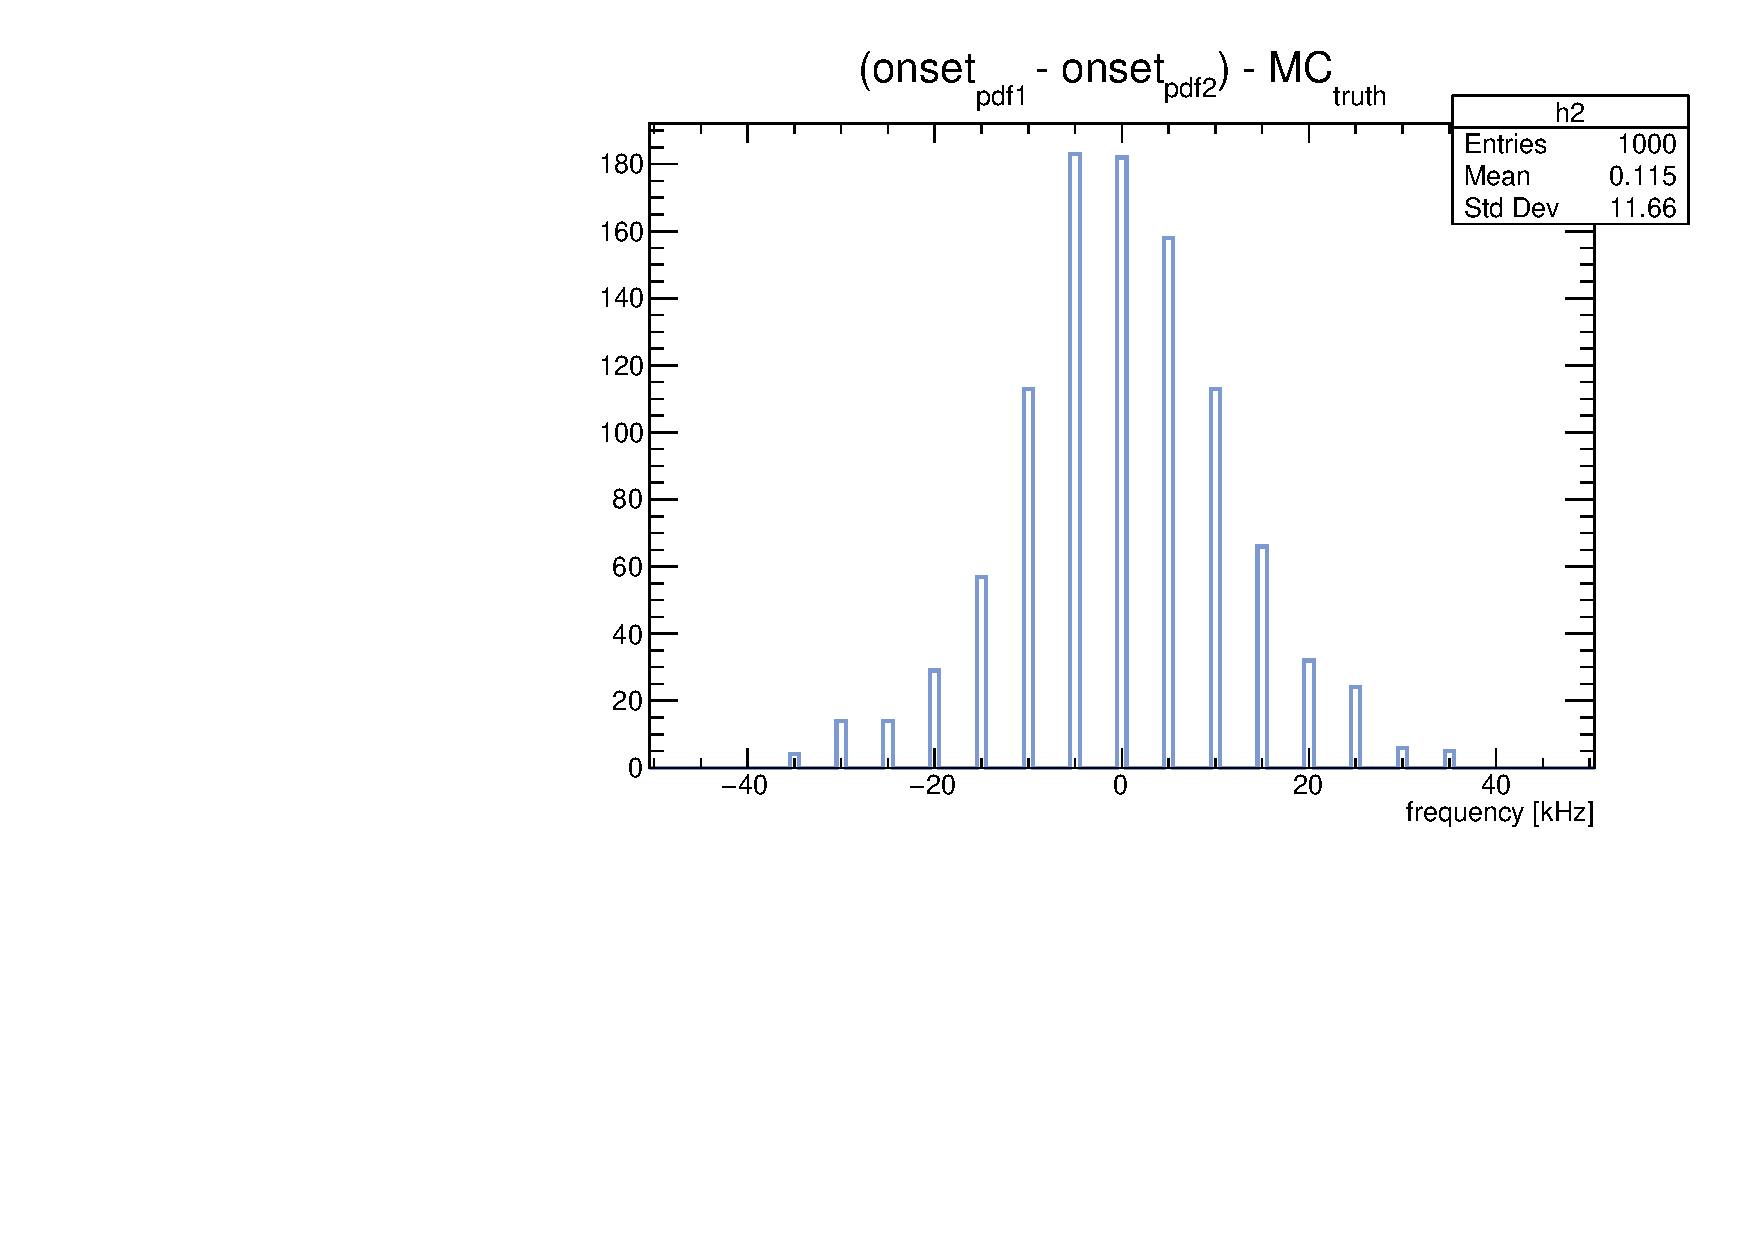
\includegraphics[width=.45\textwidth]{../Plot/delta_sumNeighbors_sigma30.pdf}}
\end{figure}
\end{frame}


\begin{frame}{Next steps}

\begin{itemize}
\item Add to the simulation the magnetic field drift
\item Systematic studies of the relative shape asymmetry for the two transitions and its effect on the onset determination.
\end{itemize}
\end{frame}

\end{document}